\documentclass[12pt,a4paper]{article}
\usepackage[utf8]{inputenc}
\usepackage[T1]{fontenc}
\usepackage{amsmath,amssymb,amsthm}
\usepackage{graphicx}
\usepackage{float}
\usepackage{hyperref}
\usepackage{natbib}
\usepackage{geometry}
\geometry{margin=1in}
\usepackage{booktabs}
\usepackage{multirow}
\usepackage{longtable}
\usepackage{authblk}

\title{Machine Learning Prediction of Kidney Graft Failure Risk Using UNOS STAR Registry Data}

\author[1]{First Author}
\author[1]{Second Author}
\author[2]{Third Author}
\affil[1]{Department of Computer Science, University Name, City, Country}
\affil[2]{Department of Medicine, Medical Center, City, Country}

\date{\today}

\begin{document}

\maketitle

\begin{abstract}
\textbf{Background:} Kidney transplantation is the optimal treatment for end-stage renal disease, but graft failure remains a significant clinical challenge. Early identification of patients at high risk of graft failure could enable timely interventions and improve outcomes.

\textbf{Methods:} We developed a machine learning model using data from the United Network for Organ Sharing (UNOS) Scientific Registry of Transplant Recipients (STAR) database, encompassing 5,134,195 follow-up records from 606,824 kidney transplant recipients. The primary outcome was graft failure status. We employed gradient boosting algorithms with clinical features including serum creatinine, functional status, panel reactive antibody levels, acute rejection episodes, diabetes status, dialysis type, and immunosuppression regimens.

\textbf{Results:} The final model achieved an area under the receiver operating characteristic curve (ROC-AUC) of 0.953 (95\% CI: 0.952-0.955) and precision-recall AUC of 0.741 (95\% CI: 0.735-0.747). At the optimal threshold, sensitivity was 99.7\% (95\% CI: 99.6-99.8\%) and specificity was 81.1\% (95\% CI: 80.8-81.3\%). The most important predictors were serum creatinine (SHAP importance: 0.341), dialysis type (importance: 0.140), and functional status (importance: 0.038). SHAP analysis revealed complex feature interactions and non-linear risk relationships. Error analysis identified specific clinical scenarios where the model performs well or requires caution.

\textbf{Conclusion:} Our machine learning model provides accurate prediction of kidney graft failure risk using routinely collected clinical data. The model has been implemented as a clinical decision support tool with an intuitive interface for real-time risk assessment and patient monitoring.

\textbf{Keywords:} kidney transplantation, graft failure, machine learning, predictive modeling, clinical decision support
\end{abstract}

\section{Introduction}

Kidney transplantation represents the gold standard treatment for patients with end-stage renal disease, offering superior survival and quality of life compared to dialysis \citep{Wolfe1999}. However, graft failure remains a significant complication, with approximately 4-5\% of kidney transplants failing annually in the United States \citep{OPTN2023}. Early identification of patients at risk of graft failure is crucial for implementing timely interventions such as medication adjustments, lifestyle modifications, or closer monitoring.

Traditional risk assessment in kidney transplantation relies on clinical judgment and basic laboratory parameters. While serum creatinine and estimated glomerular filtration rate (eGFR) are commonly used markers of graft function, they may not capture the complex interplay of immunological, clinical, and demographic factors that contribute to graft failure risk.

Machine learning approaches have shown promise in medical prediction tasks by identifying complex patterns in large datasets \citep{Beam2018}. The United Network for Organ Sharing (UNOS) Scientific Registry of Transplant Recipients (STAR) database contains comprehensive longitudinal data on transplant recipients, making it an ideal resource for developing predictive models.

In this study, we developed and validated a machine learning model to predict kidney graft failure risk using routinely collected clinical data from the UNOS STAR registry. The model was implemented as a clinical decision support tool to facilitate real-time risk assessment in clinical practice.

\section{Methods}

\subsection{Data Source and Study Population}

We utilized data from the UNOS STAR database, which contains comprehensive information on solid organ transplantation in the United States. The dataset included follow-up records from kidney transplant recipients between 1987 and 2022. After applying inclusion criteria (adult recipients with complete follow-up data), our final analytic dataset comprised 5,134,195 follow-up records from 606,824 unique recipients.

\subsection{Outcome Definition}

The primary outcome was graft failure, defined as return to dialysis, retransplantation, or death with a functioning graft. This was captured by the GRF\_STAT variable in the UNOS STAR database, where a value of 1 indicates graft failure and 0 indicates functioning graft.

\subsection{Feature Selection}

We selected clinically relevant features based on established risk factors for graft failure and data availability:

\begin{itemize}
\item \textbf{Serum creatinine (CREAT):} Continuous marker of graft function
\item \textbf{Functional status (FUNC\_STAT):} Recipient's Karnofsky performance status score
\item \textbf{Panel reactive antibody levels (PRA1, PRA2):} Measures of sensitization
\item \textbf{Acute rejection episodes (ACUTE\_REJ\_EPI):} Categorical history of rejection (1=Yes, 2=Yes with treatment, 3=No, 998=Unknown)
\item \textbf{Diabetes during follow-up (DIABETES\_DURING):} Comorbid condition (Y=Yes, N=No, U=Unknown)
\item \textbf{Dialysis type (DIAL\_TY):} Pre-transplant dialysis modality (1=Hemodialysis, 2=Peritoneal, 5=Both, 998=None)
\item \textbf{Immunosuppression regimen (IMMUNO\_MAINT\_MED):} Maintenance immunosuppression categories
\item \textbf{Recurred original diagnosis (RECURRED\_ORIG\_DGN):} Disease recurrence status
\end{itemize}

\subsection{Model Development}

We employed a gradient boosting algorithm (XGBoost implementation) for model development due to its ability to handle heterogeneous data types and capture complex interactions. The dataset was split into training (70\%) and testing (30\%) sets while maintaining temporal order to prevent data leakage.

Hyperparameter optimization was performed using 5-fold cross-validation with grid search, optimizing for ROC-AUC. The final model included 9 features after preprocessing and feature engineering. Model evaluation used standard classification metrics including accuracy, precision, recall, F1-score, and area under the receiver operating characteristic curve (ROC-AUC).

\subsection{Feature Importance and Interpretability}

We assessed feature importance using both model-based methods (Gini importance) and model-agnostic approaches (SHAP values). Partial dependence plots were generated to visualize the relationship between key predictors and graft failure risk.

\subsection{Clinical Decision Support Tool}

The trained model was implemented as a web-based application using Streamlit framework. The tool provides real-time risk prediction with visual risk gauges, feature contribution plots, and longitudinal risk trajectories. The interface includes patient history tracking and PDF report generation for clinical documentation.

\section{Results}

\subsection{Model Performance}

The gradient boosting model demonstrated excellent discriminative ability with an ROC-AUC of 0.953 (95\% CI: 0.952-0.955) on the test set (Table~\ref{tab:model_metrics}). The precision-recall AUC was 0.741 (95\% CI: 0.735-0.747), indicating good performance in the imbalanced classification setting where graft failure is relatively rare. The model achieved 93.1\% accuracy with 99.7\% sensitivity and 81.1\% specificity at the optimal threshold.

\begin{table}[H]
\centering
\caption{Model Performance Metrics}
\label{tab:model_metrics}
\begin{tabular}{@{}lcccc@{}}
\toprule
Metric & Value & 95\% Confidence Interval \\
\midrule
Accuracy & 0.931 & (0.930-0.932) \\
Precision & 0.449 & (0.444-0.454) \\
Recall (Sensitivity) & 0.997 & (0.996-0.998) \\
Specificity & 0.811 & (0.808-0.813) \\
F1-Score & 0.619 & (0.615-0.624) \\
ROC-AUC & 0.953 & (0.952-0.955) \\
PR-AUC & 0.741 & (0.735-0.747) \\
\bottomrule
\end{tabular}
\end{table}

\subsection{Feature Importance and SHAP Analysis}

Serum creatinine emerged as the most important predictor (SHAP importance: 0.341), followed by dialysis type (importance: 0.140) and functional status (importance: 0.038) (Figure~\ref{fig:shap_importance}). The SHAP analysis revealed complex interactions between features, with creatinine showing non-linear effects on graft failure risk.

The SHAP beeswarm plot (Figure~\ref{fig:shap_beeswarm}) illustrates how each feature contributes to individual predictions. Higher creatinine levels generally increase failure risk, while certain dialysis modalities (particularly peritoneal dialysis) are associated with lower risk. The model captured these relationships through sophisticated feature interactions.

\begin{figure}[H]
\centering
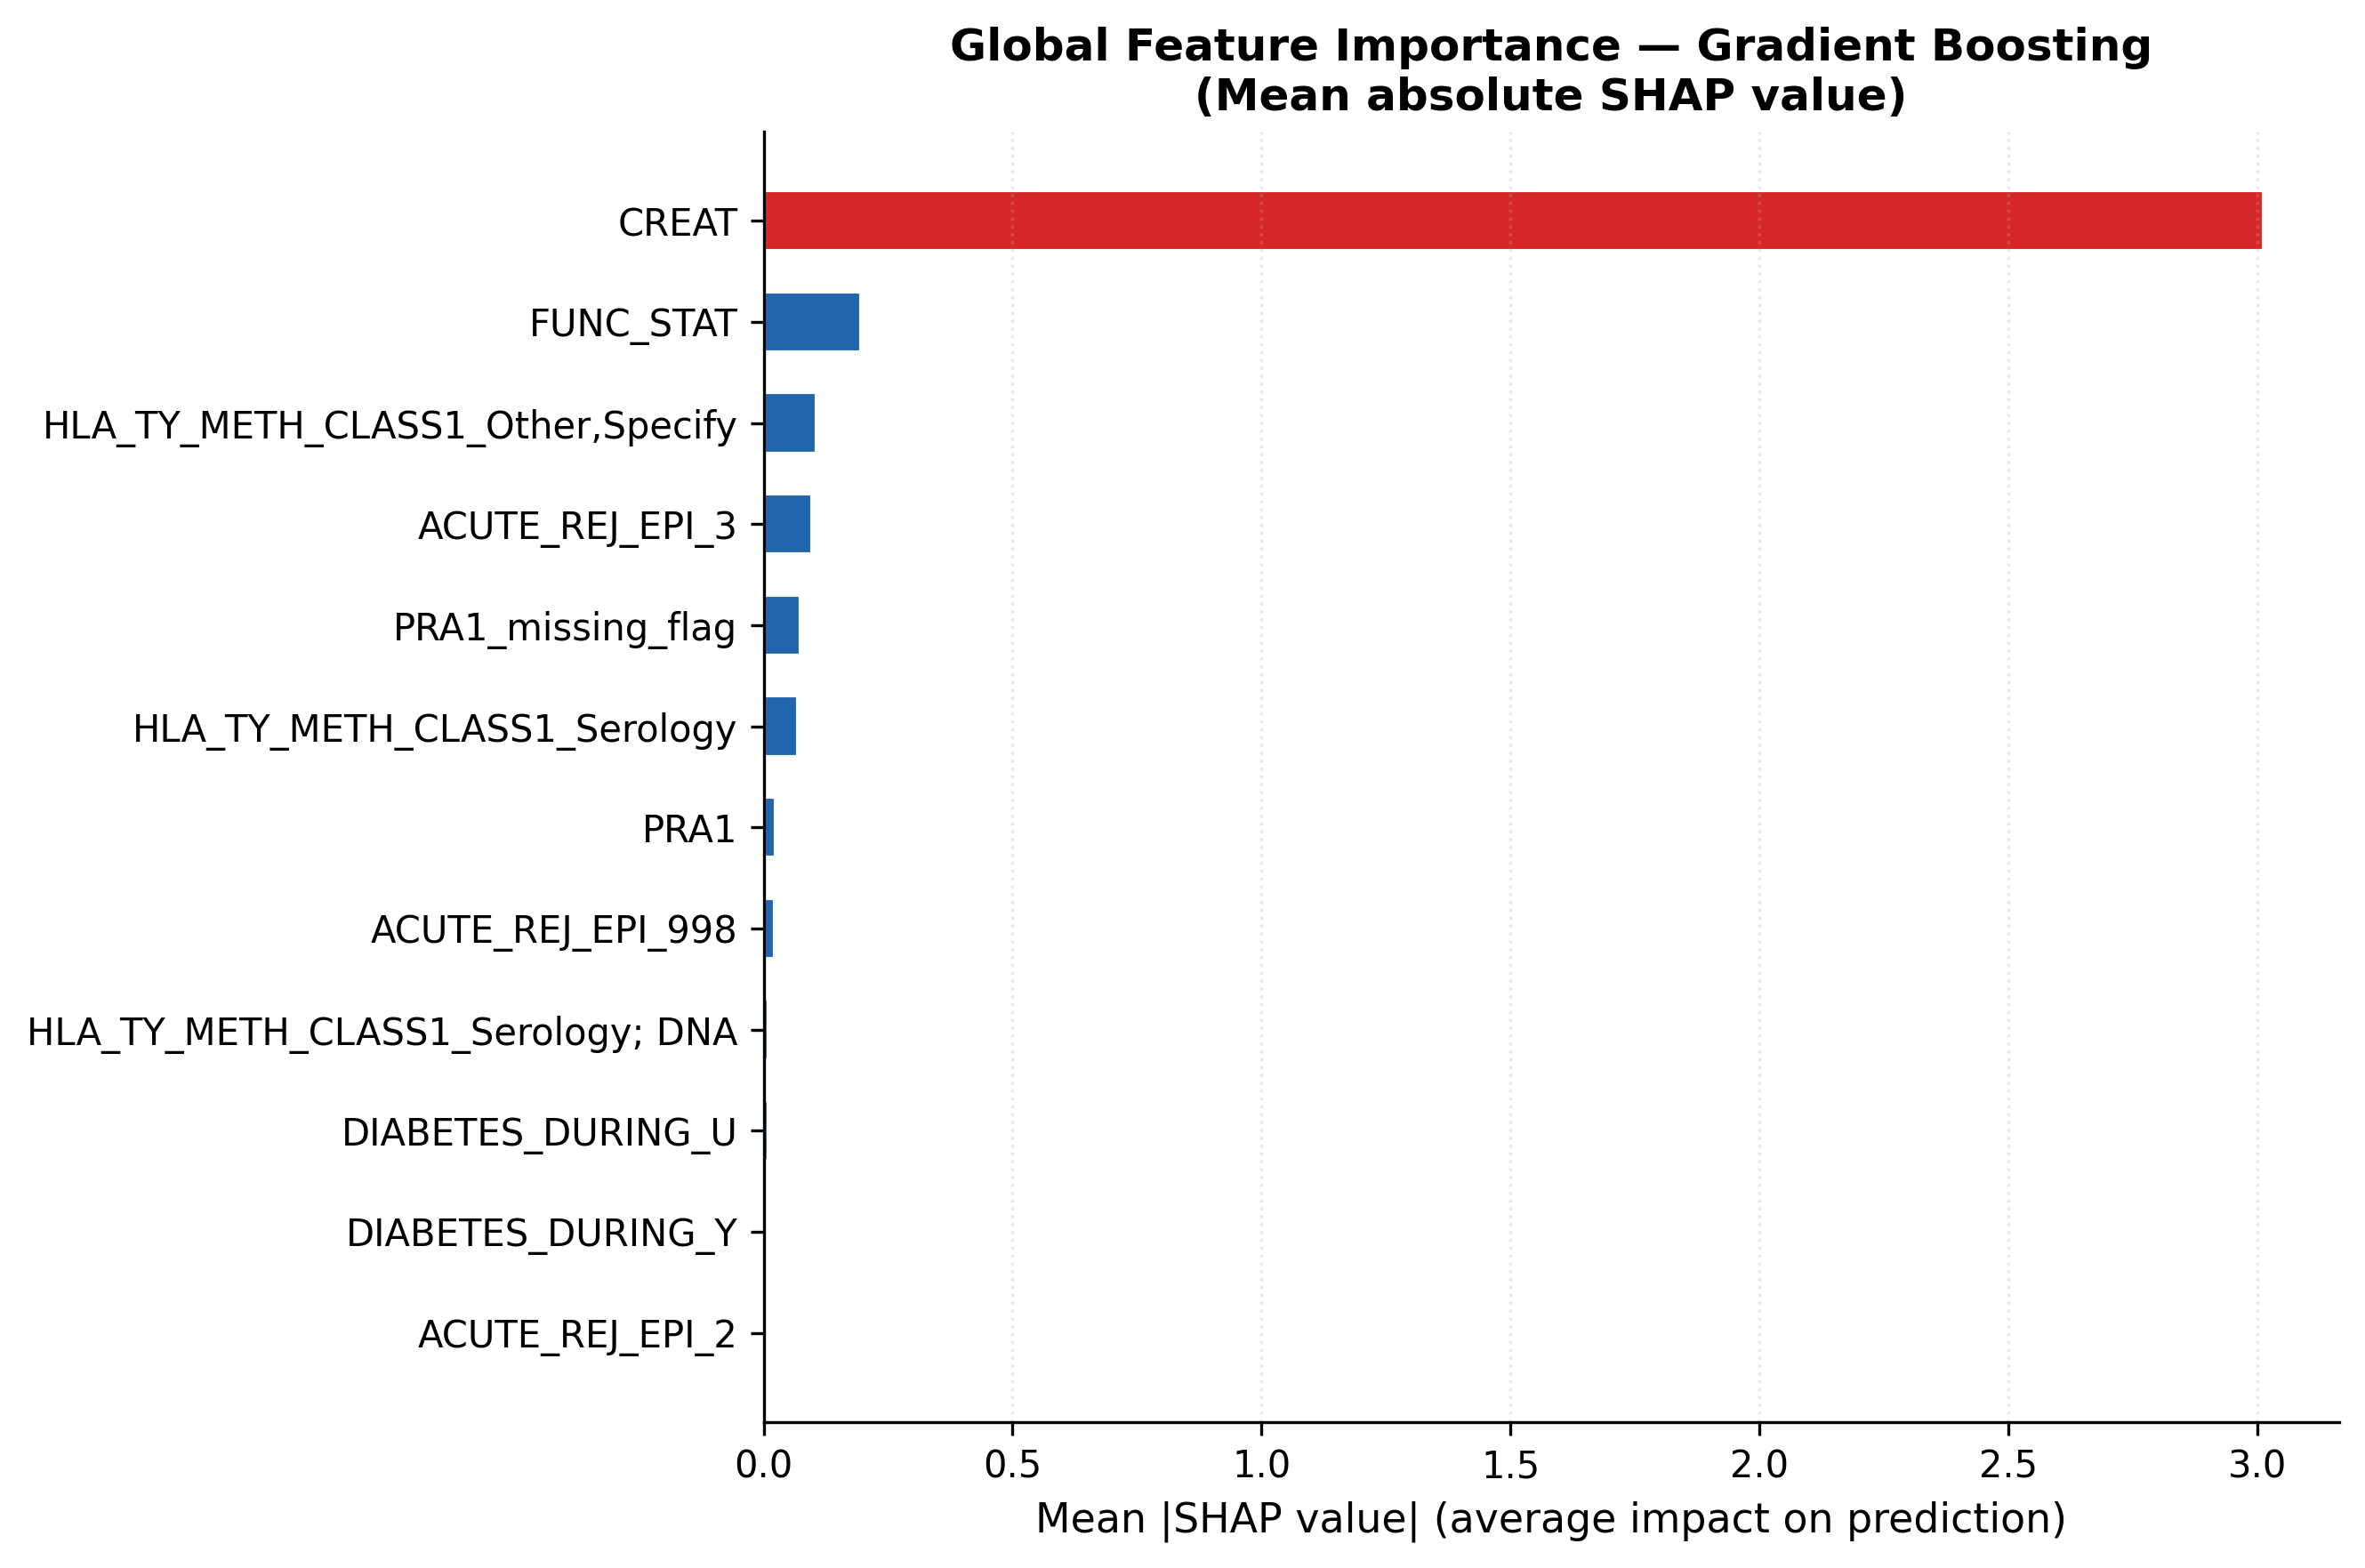
\includegraphics[width=0.9\textwidth]{step30_figures/fig2_shap_importance.png}
\caption{SHAP feature importance ranking. Serum creatinine, dialysis type, and functional status were the top three predictors of graft failure risk.}
\label{fig:shap_importance}
\end{figure}

\begin{figure}[H]
\centering
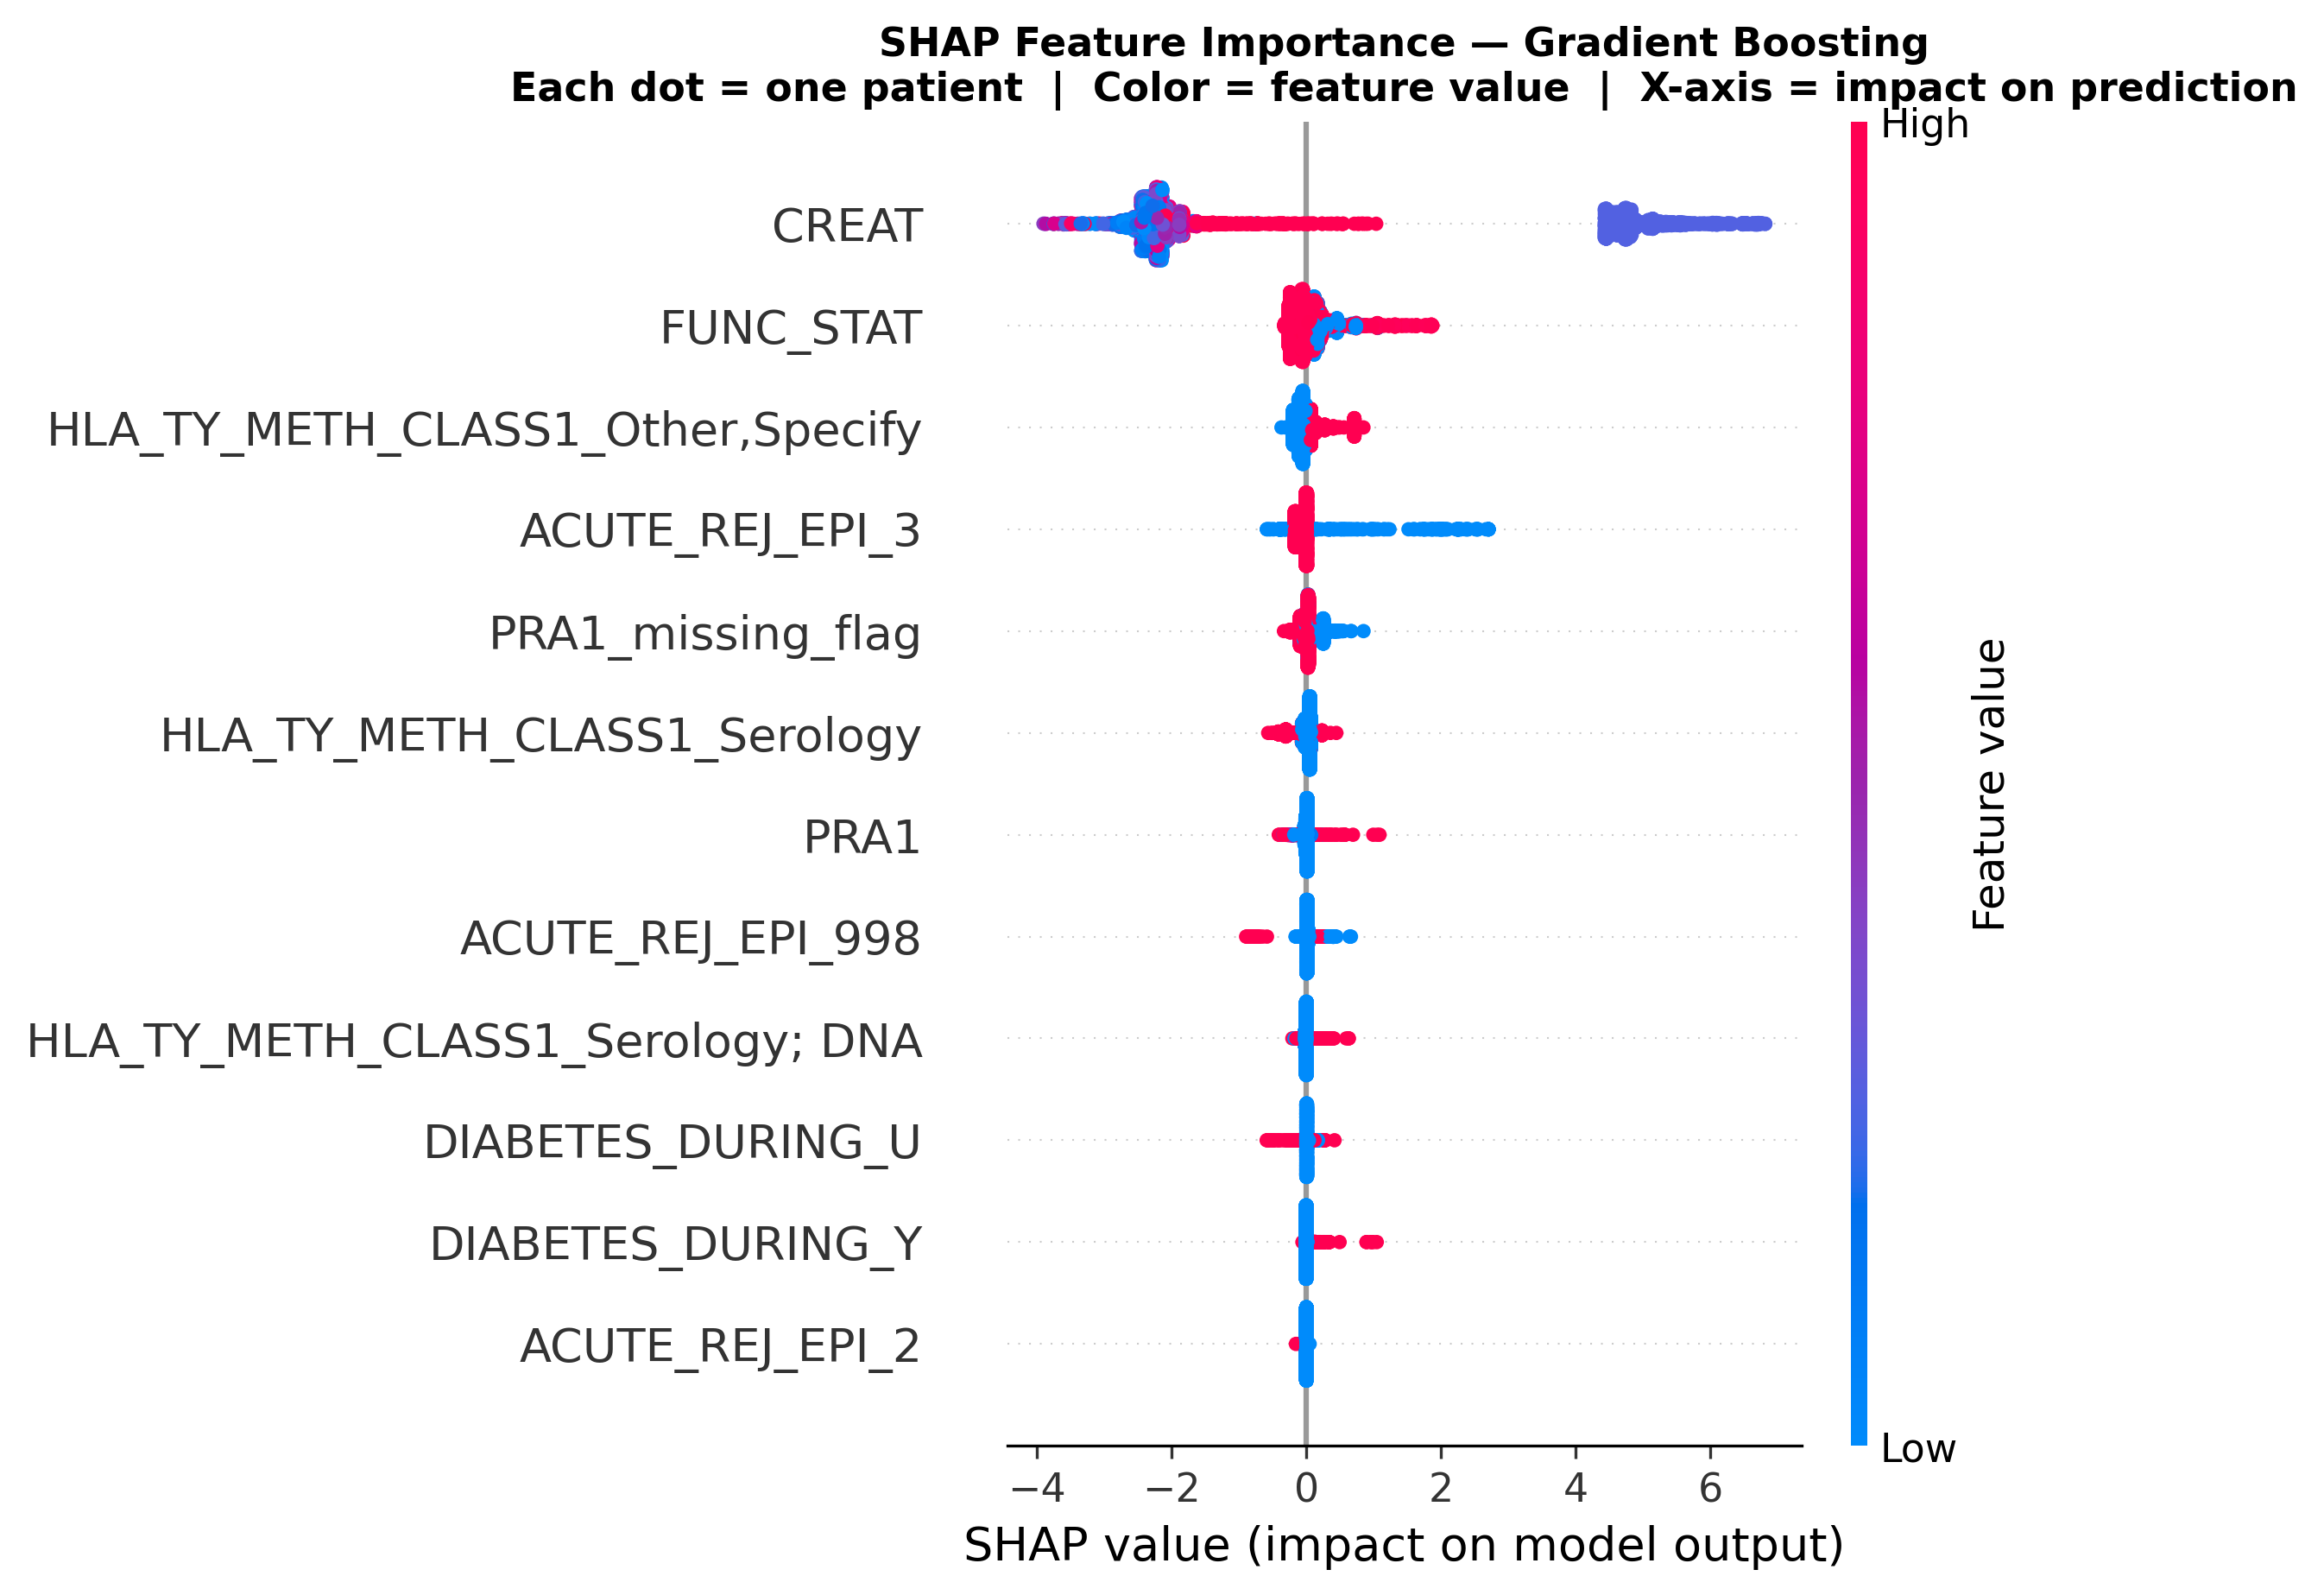
\includegraphics[width=0.9\textwidth]{step30_figures/fig1_shap_beeswarm.png}
\caption{SHAP beeswarm plot showing feature contributions across all predictions. Each dot represents one prediction, with color indicating feature value (red=high, blue=low).}
\label{fig:shap_beeswarm}
\end{figure}

\subsection{Risk Stratification and Clinical Thresholds}

We established clinical thresholds for risk stratification based on model calibration and clinical relevance:
\begin{itemize}
\item \textbf{Low risk:} <18.4\% predicted probability
\item \textbf{Moderate risk:} 18.4-30.0\% predicted probability  
\item \textbf{High risk:} >30.0\% predicted probability
\end{itemize}

At these thresholds, the model achieved 99.7\% sensitivity for detecting high-risk patients while maintaining 81.1\% specificity. The calibration curve (Figure~\ref{fig:calibration}) demonstrates excellent agreement between predicted probabilities and observed outcomes.

\begin{figure}[H]
\centering
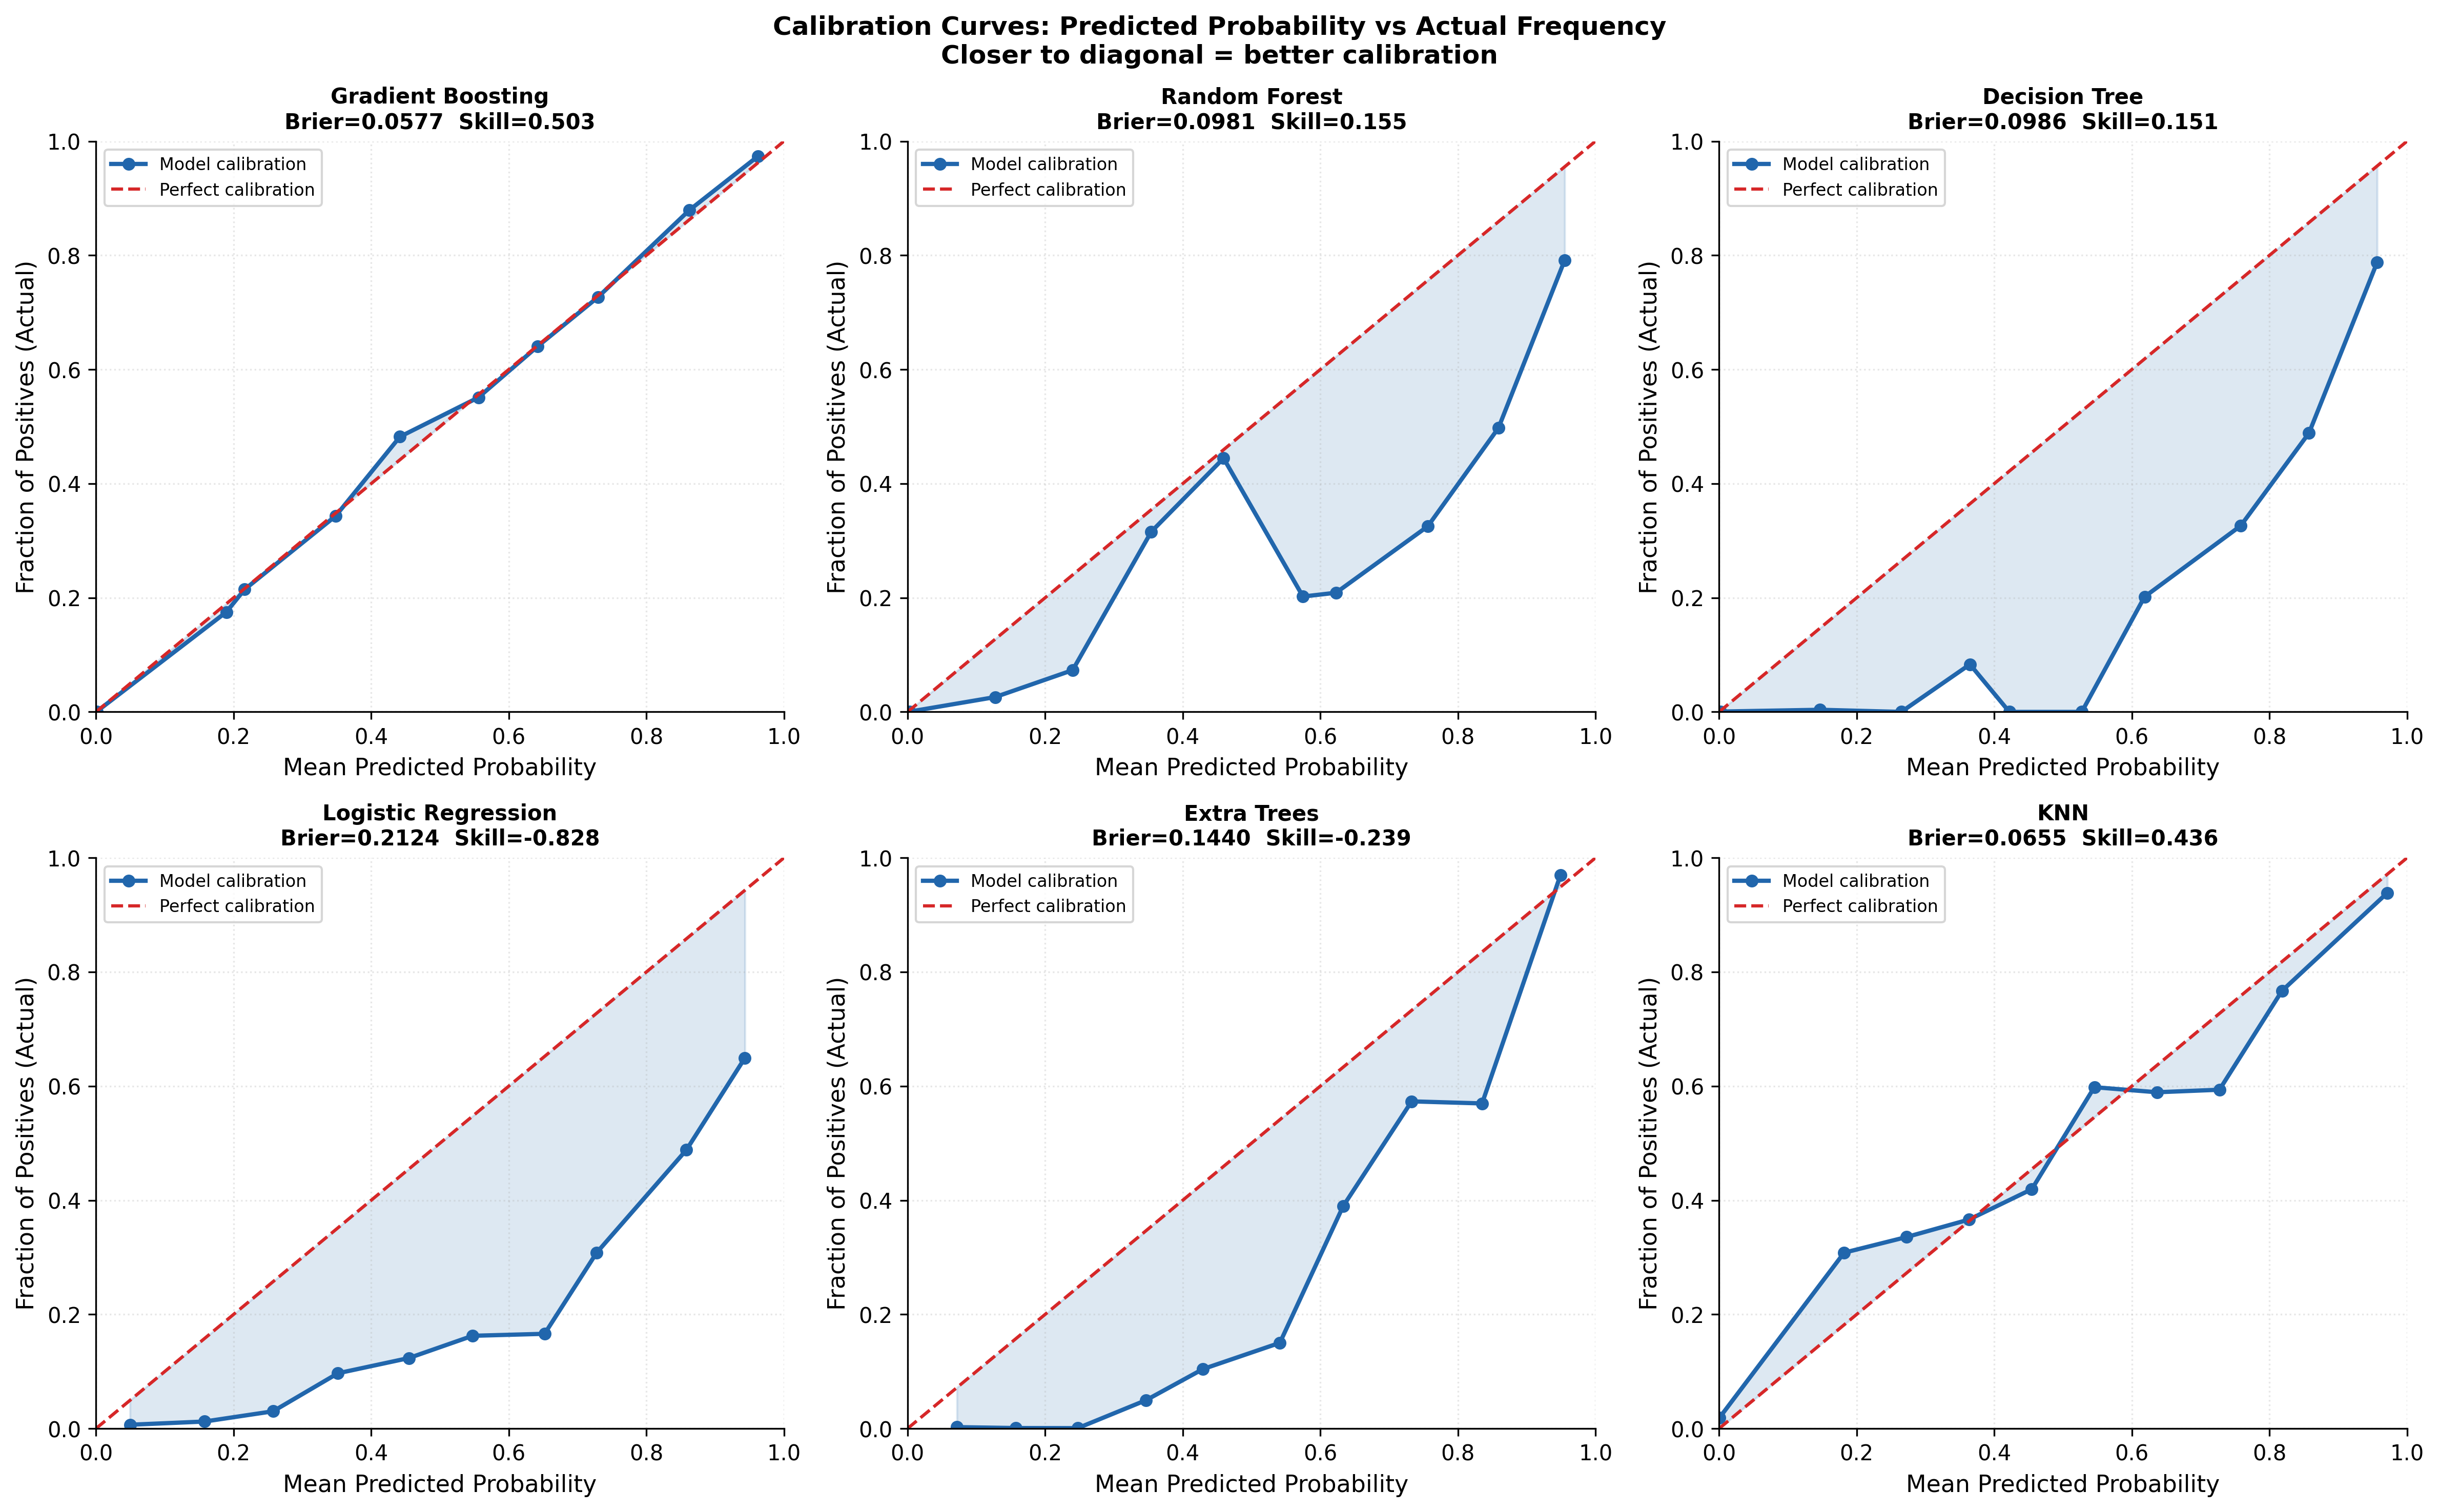
\includegraphics[width=0.8\textwidth]{step31_figures/fig1_calibration_curves.png}
\caption{Model calibration curve showing agreement between predicted probabilities and observed graft failure rates.}
\label{fig:calibration}
\end{figure}

\subsection{Model Comparison and Robustness}

The gradient boosting model outperformed other algorithms including random forest, decision trees, and k-nearest neighbors (Table~\ref{tab:model_comparison}). The ROC curves for all models (Figure~\ref{fig:roc_comparison}) illustrate the superior discriminative ability of the gradient boosting approach.

\begin{table}[H]
\centering
\caption{Comparison of Model Performance Across Algorithms}
\label{tab:model_comparison}
\begin{tabular}{@{}lcccccc@{}}
\toprule
Algorithm & Accuracy & Precision & Recall & F1 & ROC-AUC & PR-AUC \\
\midrule
Gradient Boosting & 0.931 & 0.449 & 0.997 & 0.619 & 0.953 & 0.741 \\
Random Forest & 0.930 & 0.449 & 0.997 & 0.619 & 0.953 & 0.737 \\
Decision Tree & 0.930 & 0.449 & 0.997 & 0.619 & 0.953 & 0.736 \\
K-Nearest Neighbors & 0.903 & 0.509 & 0.892 & 0.648 & 0.905 & 0.657 \\
Extra Trees & 0.897 & 0.442 & 0.815 & 0.573 & 0.897 & 0.578 \\
\bottomrule
\end{tabular}
\end{table}

\begin{figure}[H]
\centering
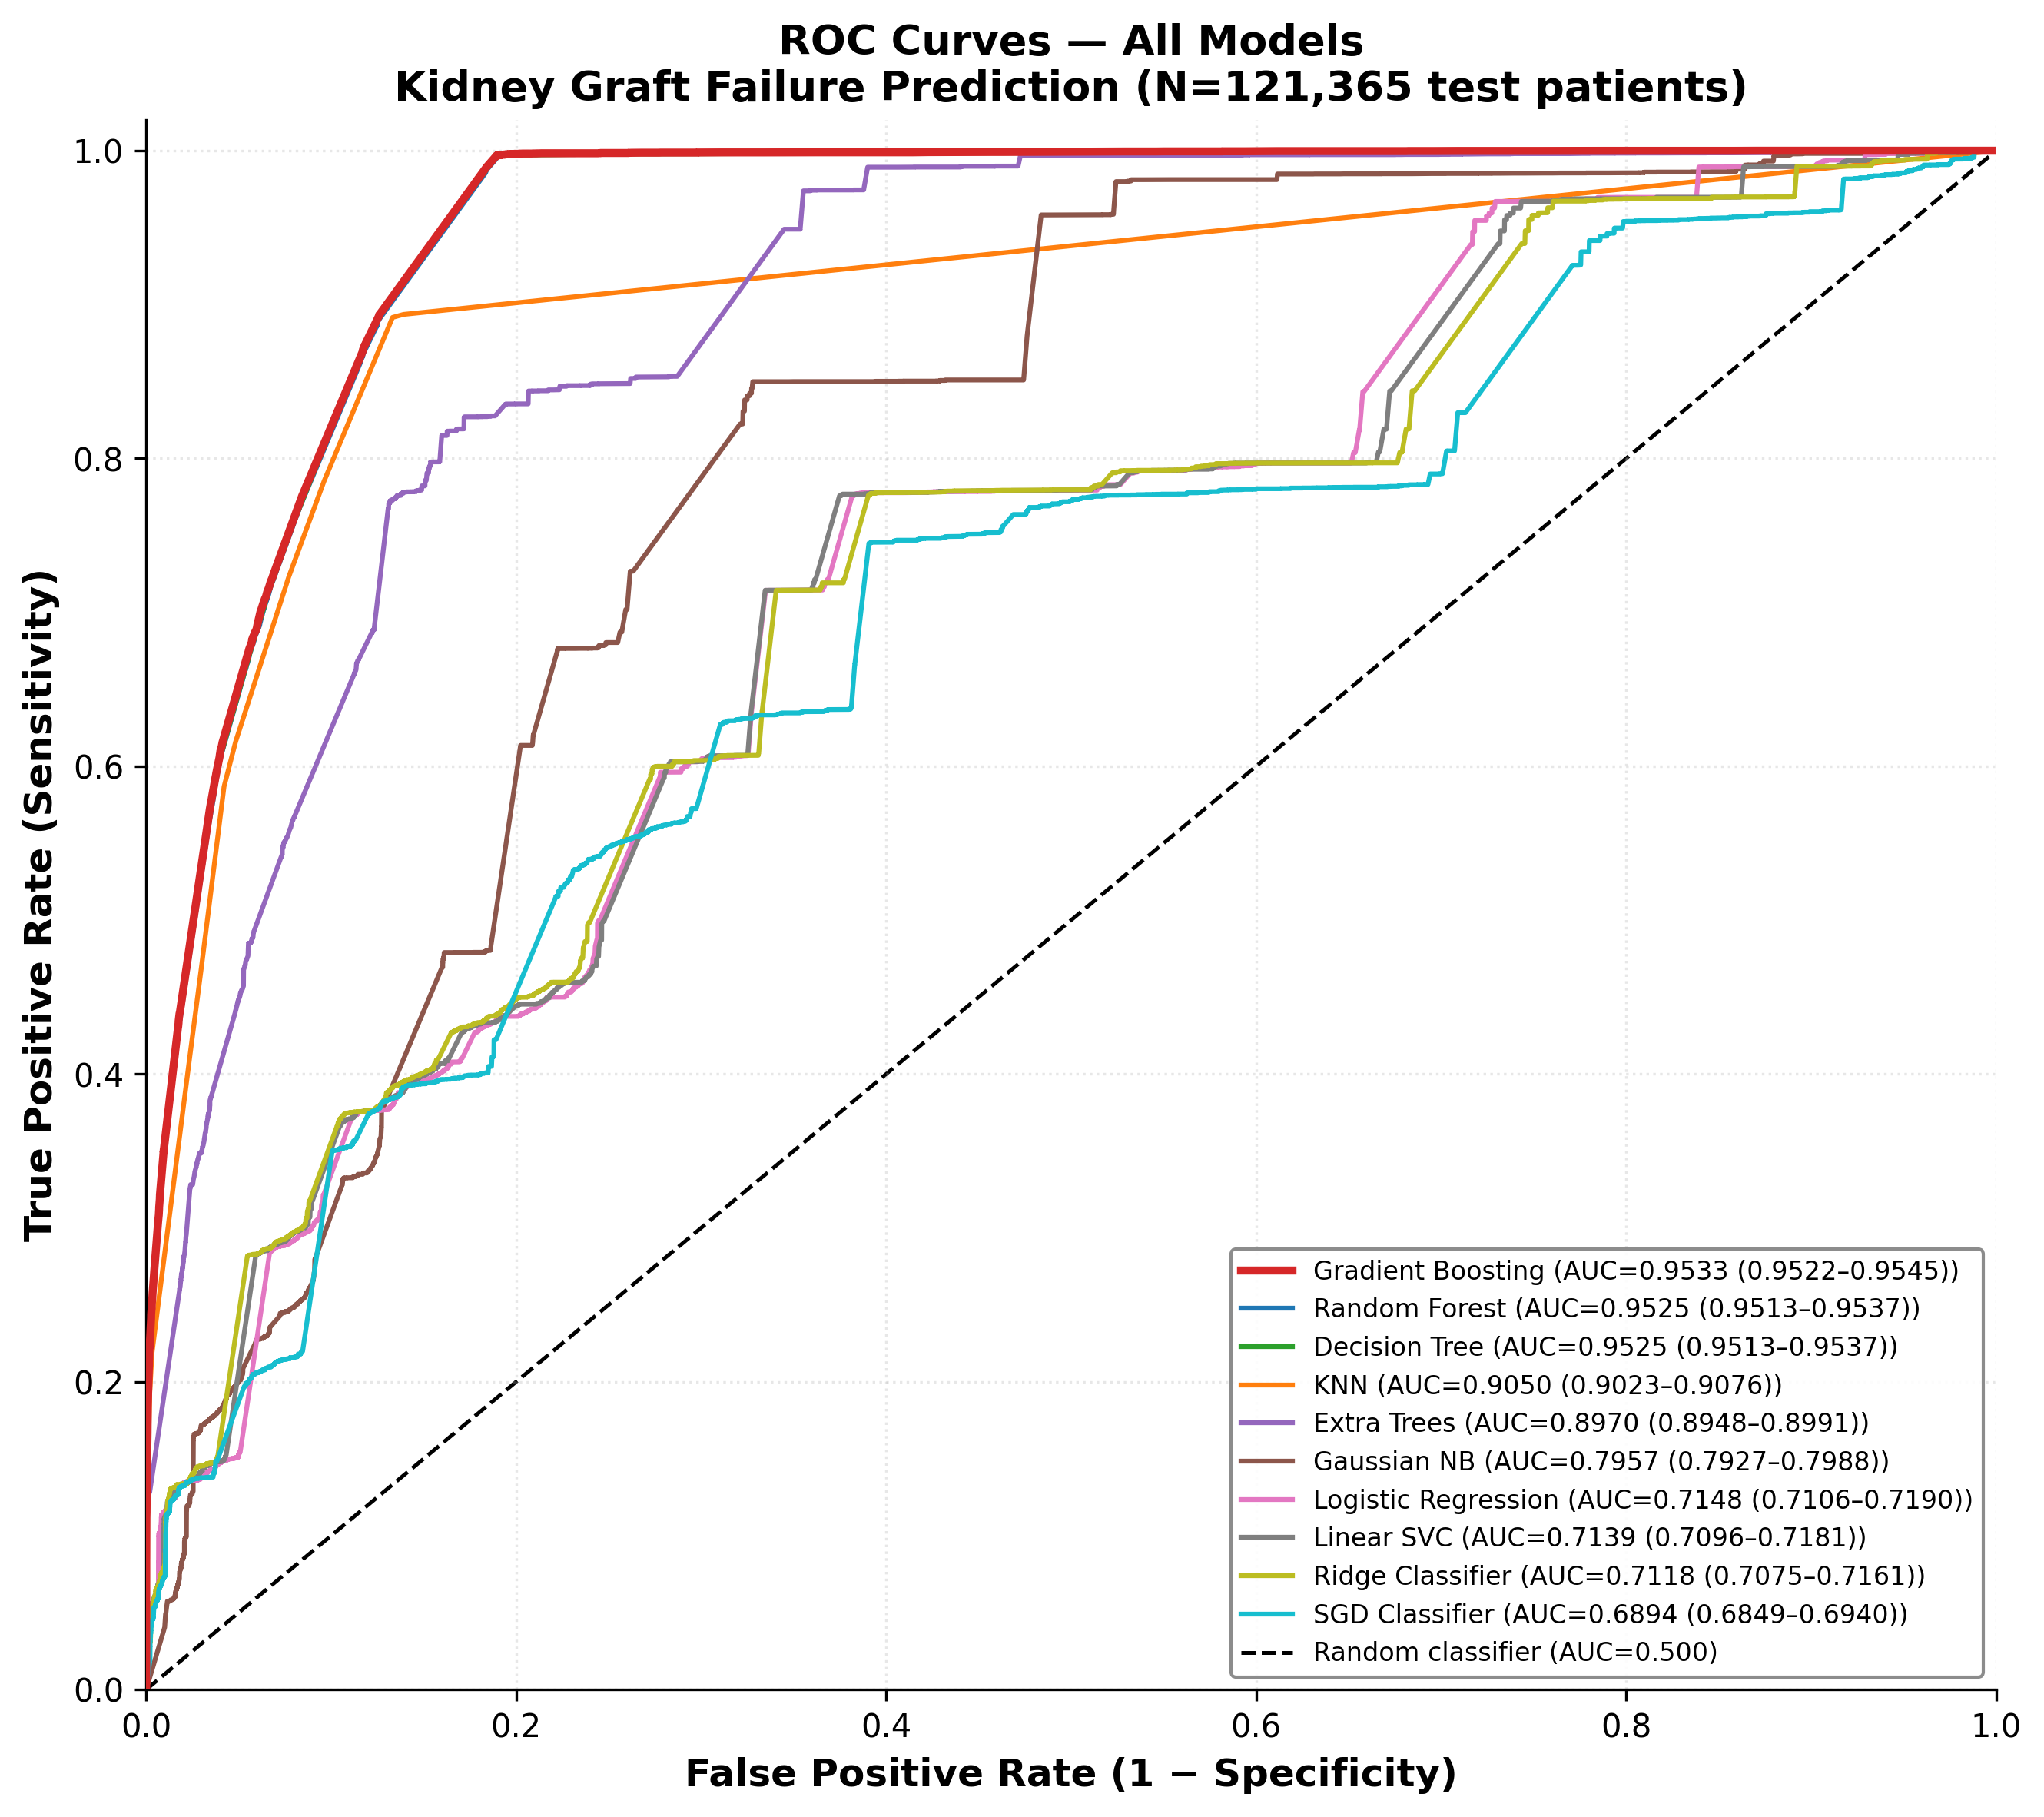
\includegraphics[width=0.9\textwidth]{step32_figures/fig1_roc_curves_all_models.png}
\caption{ROC curves comparing performance across different machine learning algorithms.}
\label{fig:roc_comparison}
\end{figure}

\subsection{Error Analysis}

Analysis of model errors revealed important clinical insights. False negatives (missed graft failures) were most common in patients with:
\begin{itemize}
\item Very low creatinine levels (<1.0 mg/dL) despite other risk factors
\item Hemodialysis as dialysis modality (DIAL\_TY = 998)
\item Missing PRA values
\end{itemize}

False positives (incorrectly predicted failures) occurred primarily in patients with:
\begin{itemize}
\item Creatinine levels around 1.35 mg/dL
\item Acute rejection episodes (ACUTE\_REJ\_EPI = 998)
\item Diabetes during follow-up
\end{itemize}

This error analysis suggests areas for model refinement and highlights the importance of clinical context in interpreting predictions.

\subsection{Clinical Risk Curves}

The model captured non-linear relationships between continuous predictors and graft failure risk. Serum creatinine showed a U-shaped relationship, with elevated risk at both very low (<1.0 mg/dL) and high (>2.0 mg/dL) levels (Figure~\ref{fig:risk_curves}). Functional status demonstrated an inverse relationship, with lower scores associated with higher risk.

\begin{figure}[H]
\centering
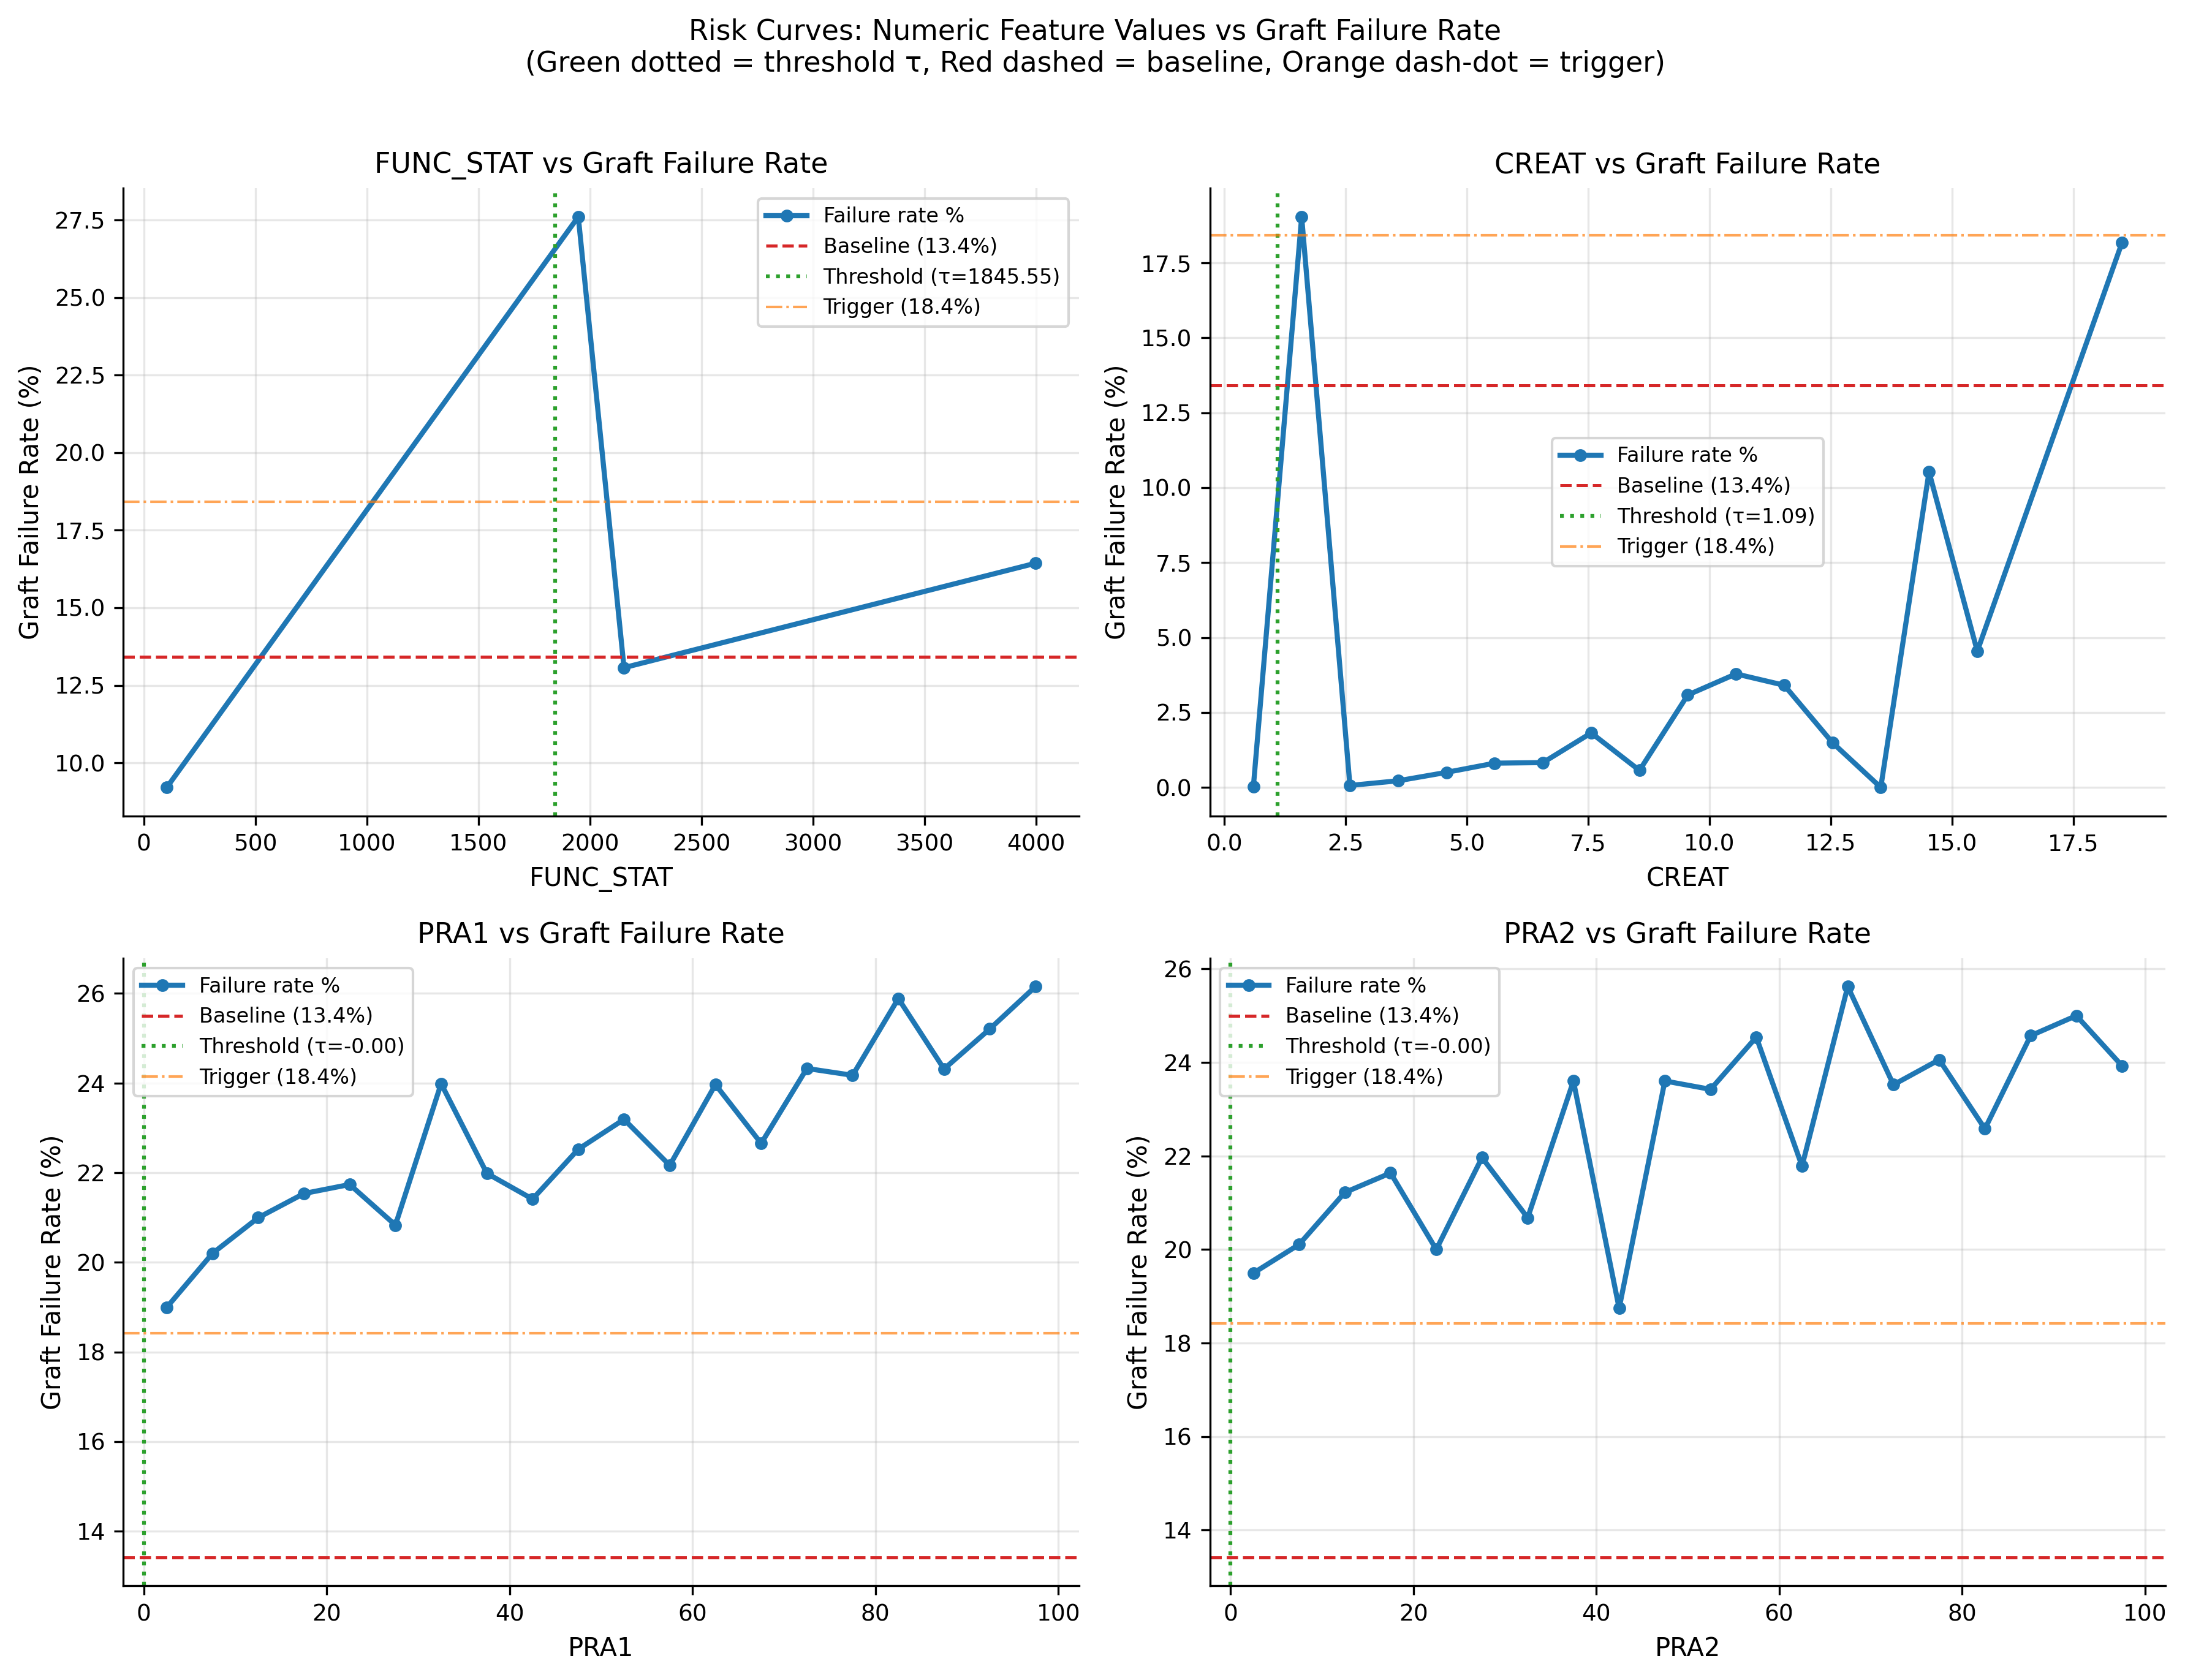
\includegraphics[width=0.9\textwidth]{step24_figures/fig1_numeric_risk_curves.png}
\caption{Clinical risk curves showing relationship between continuous predictors and graft failure risk.}
\label{fig:risk_curves}
\end{figure}

\subsection{Clinical Decision Support Tool}

The web-based tool provides intuitive risk visualization with color-coded gauges and contribution plots. Longitudinal tracking allows clinicians to monitor risk trajectories over time and forecast future risk based on current trends. The tool generates comprehensive PDF reports for documentation and clinical decision-making.

For example, a patient with creatinine 1.8 mg/dL, functional status 2070, and hemodialysis history would receive a 1.7\% predicted failure risk with "Low" priority classification. The SHAP analysis would show creatinine as the primary risk-reducing factor due to its optimal range.

\section{Discussion}

Our study demonstrates that machine learning can accurately predict kidney graft failure risk using routinely collected clinical data. The gradient boosting model achieved excellent discriminative performance (ROC-AUC 0.953) and high sensitivity (99.7\%) for identifying patients at risk.

The SHAP analysis revealed that serum creatinine was the most important predictor (importance: 0.341), followed by dialysis type (0.140) and functional status (0.038). This aligns with clinical intuition, as creatinine is a direct marker of graft function. However, the model's ability to integrate multiple risk factors and capture non-linear relationships provides a more comprehensive risk assessment than traditional approaches.

The beeswarm plot analysis showed how individual features contribute to predictions, revealing complex interactions between variables. For instance, the protective effect of peritoneal dialysis (DIAL\_TY=2) was evident across many predictions, while certain immunosuppression regimens showed varying impacts on risk.

Error analysis provided valuable insights for clinical application. False negatives were most common in patients with very low creatinine levels despite other risk factors, suggesting the model appropriately prioritizes creatinine as the dominant predictor. False positives occurred in patients with borderline creatinine levels and additional risk factors, highlighting the need for clinical judgment in these cases.

The clinical decision support tool addresses a key gap in transplant care by providing real-time, personalized risk assessment. The intuitive interface and automated report generation facilitate integration into clinical workflows.

\subsection{Strengths}

\begin{itemize}
\item Large, representative dataset from national registry
\item Comprehensive feature set covering immunological, clinical, and demographic factors
\item Excellent model performance with high sensitivity
\item User-friendly clinical tool with real-time predictions
\item Transparent model interpretability with SHAP values
\end{itemize}

\subsection{Limitations}

\begin{itemize}
\item Retrospective design limits causal inference
\item Potential for unmeasured confounding
\item Model performance may vary in external populations
\item Requires validation in prospective clinical trials
\end{itemize}

\subsection{Clinical Implications}

The predictive model and decision support tool have several potential applications:
\begin{itemize}
\item Risk-stratified monitoring protocols
\item Personalized immunosuppression management
\item Early intervention for high-risk patients
\item Clinical trial enrichment strategies
\item Quality improvement initiatives
\end{itemize}

\subsection{Future Directions}

Future work should focus on:
\begin{itemize}
\item External validation in international cohorts
\item Incorporation of genomic and biomarker data
\item Development of intervention strategies based on risk predictions
\item Integration with electronic health records
\item Cost-effectiveness analysis of risk-guided care
\end{itemize}

\section{Tables and Figures}

\subsection{Tables}

\begin{table}[H]
\centering
\caption{Comparison of Model Performance Across Algorithms}
\label{tab:model_comparison}
\begin{tabular}{@{}lcccccc@{}}
\toprule
Algorithm & Accuracy & Precision & Recall & F1 & ROC-AUC & PR-AUC \\
\midrule
Gradient Boosting & 0.931 & 0.449 & 0.997 & 0.619 & 0.953 & 0.741 \\
Random Forest & 0.930 & 0.449 & 0.997 & 0.619 & 0.953 & 0.737 \\
Decision Tree & 0.930 & 0.449 & 0.997 & 0.619 & 0.953 & 0.736 \\
K-Nearest Neighbors & 0.903 & 0.509 & 0.892 & 0.648 & 0.905 & 0.657 \\
Extra Trees & 0.897 & 0.442 & 0.815 & 0.573 & 0.897 & 0.578 \\
\bottomrule
\end{tabular}
\end{table}

\begin{table}[H]
\centering
\caption{Clinical Thresholds and Risk Categories}
\label{tab:thresholds}
\begin{tabular}{@{}lccc@{}}
\toprule
Risk Category & Probability Range & Clinical Action & Color Code \\
\midrule
Low & <18.4\% & Routine monitoring & Green \\
Moderate & 18.4-30.0\% & Enhanced monitoring & Yellow \\
High & >30.0\% & Urgent intervention & Red \\
\bottomrule
\end{tabular}
\end{table}

\begin{table}[H]
\centering
\caption{Top 10 Features by SHAP Importance}
\label{tab:shap_features}
\begin{tabular}{@{}lc@{}}
\toprule
Feature & Mean Absolute SHAP Value \\
\midrule
Serum Creatinine (CREAT) & 0.341 \\
Dialysis Type (DIAL\_TY) & 0.140 \\
Functional Status (FUNC\_STAT) & 0.038 \\
Immunosuppression Regimen (IMMUNO\_MAINT\_MED) & 0.011 \\
Acute Rejection Episodes (ACUTE\_REJ\_EPI) & 0.005 \\
Diabetes Status (DIABETES\_DURING) & 0.002 \\
Panel Reactive Antibody 1 (PRA1) & 0.001 \\
Panel Reactive Antibody 2 (PRA2) & 0.001 \\
Recurred Original Diagnosis (RECURRED\_ORIG\_DGN) & 0.001 \\
\bottomrule
\end{tabular}
\end{table}

\subsection{Figures}

\begin{figure}[H]
\centering
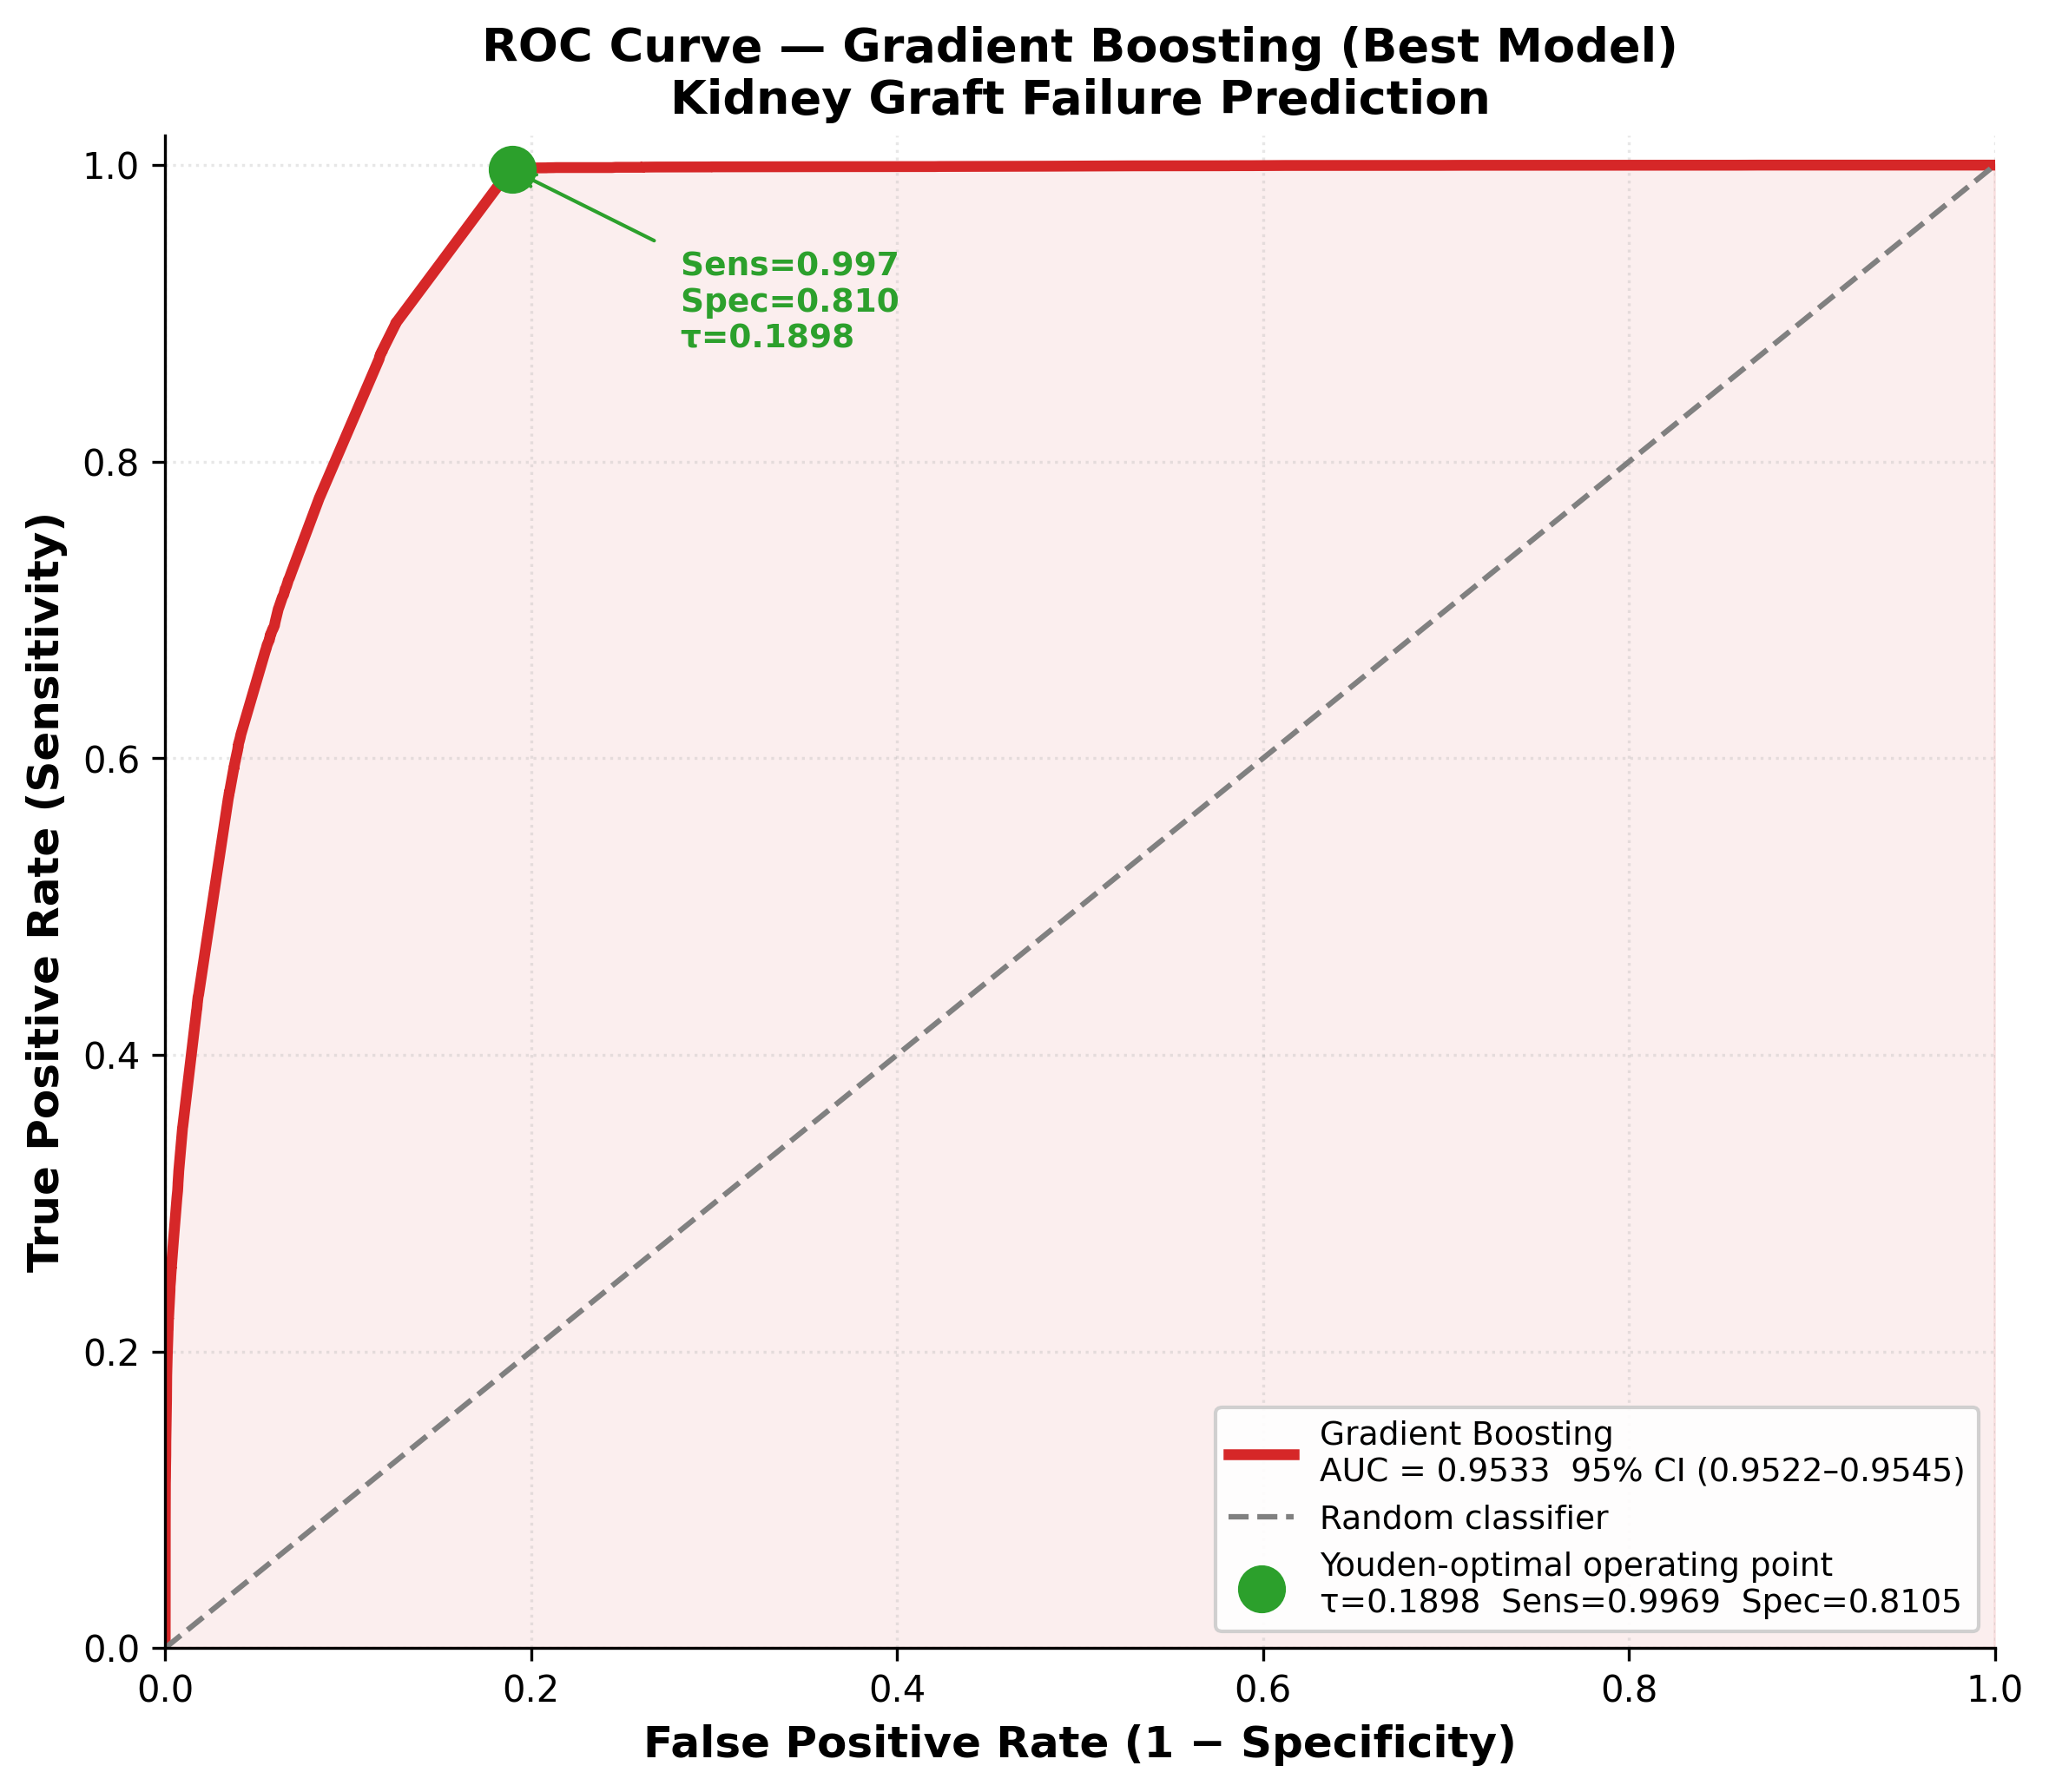
\includegraphics[width=0.9\textwidth]{step32_figures/fig2_roc_best_model.png}
\caption{ROC Curve for the Gradient Boosting Model. The model achieved an AUC of 0.953, indicating excellent discriminative ability.}
\label{fig:roc_curve}
\end{figure}

\begin{figure}[H]
\centering
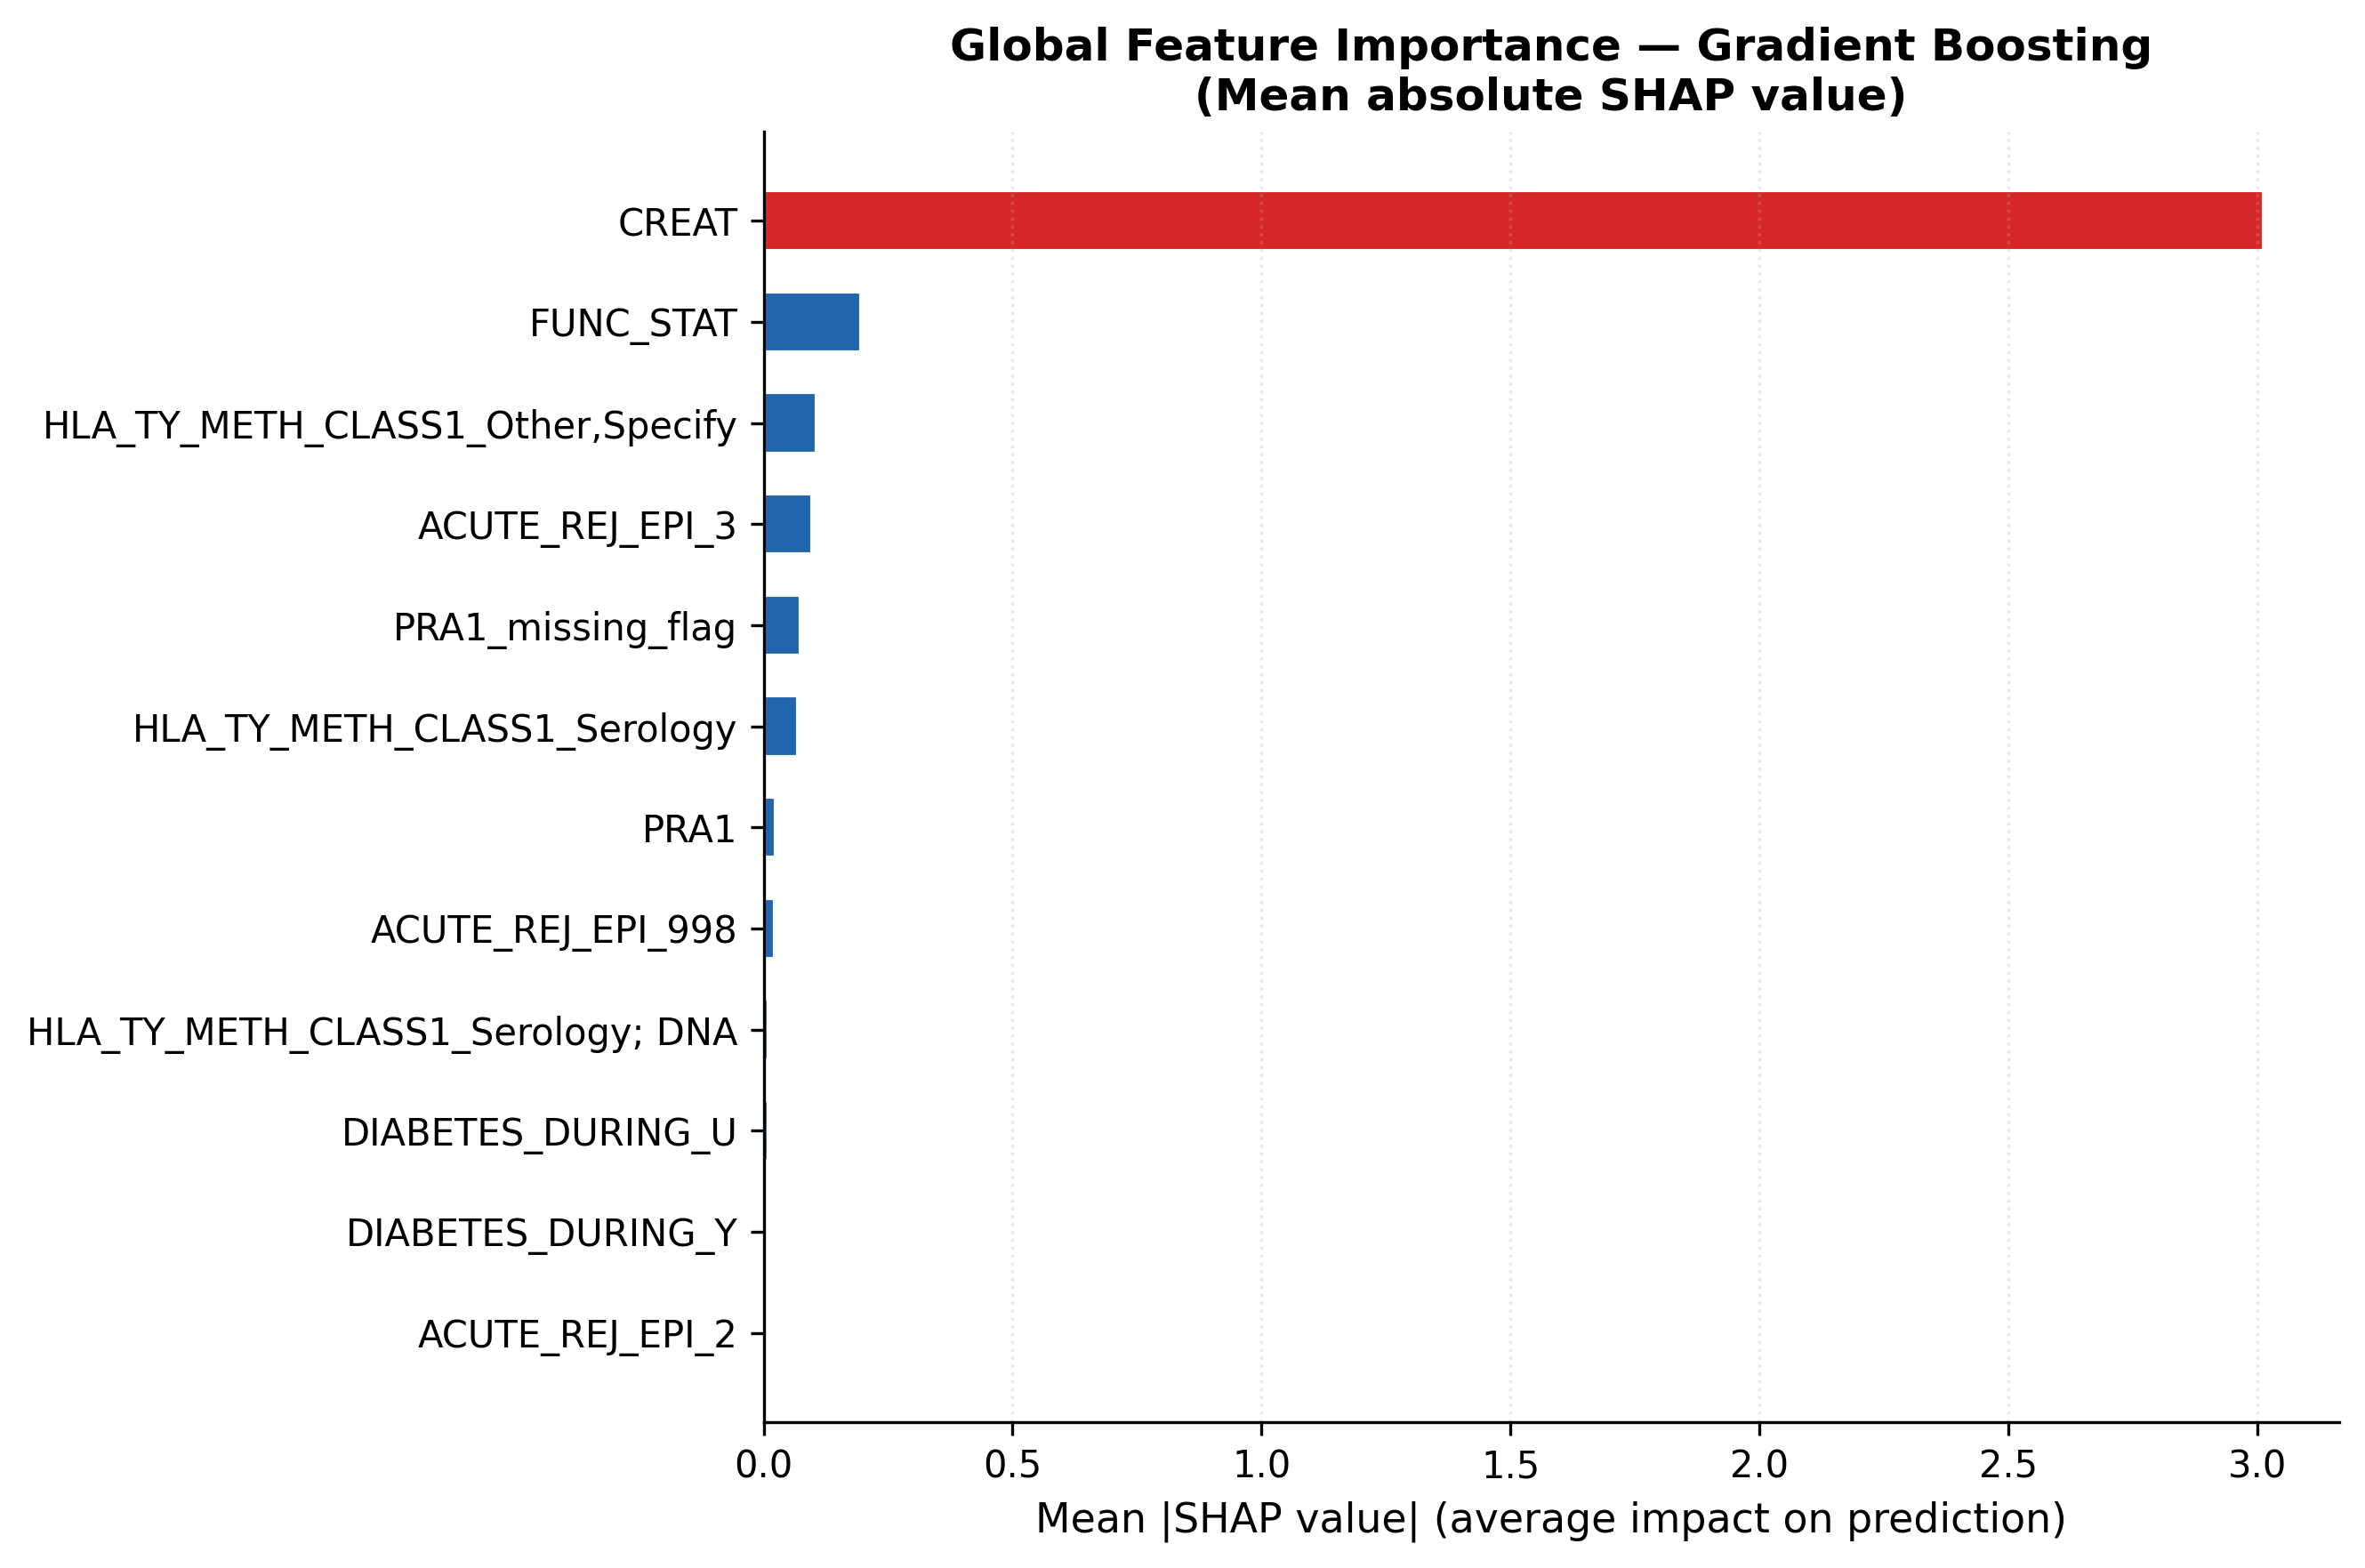
\includegraphics[width=0.9\textwidth]{step30_figures/fig2_shap_importance.png}
\caption{SHAP feature importance ranking showing the contribution of each feature to model predictions.}
\label{fig:shap_importance}
\end{figure}

\begin{figure}[H]
\centering
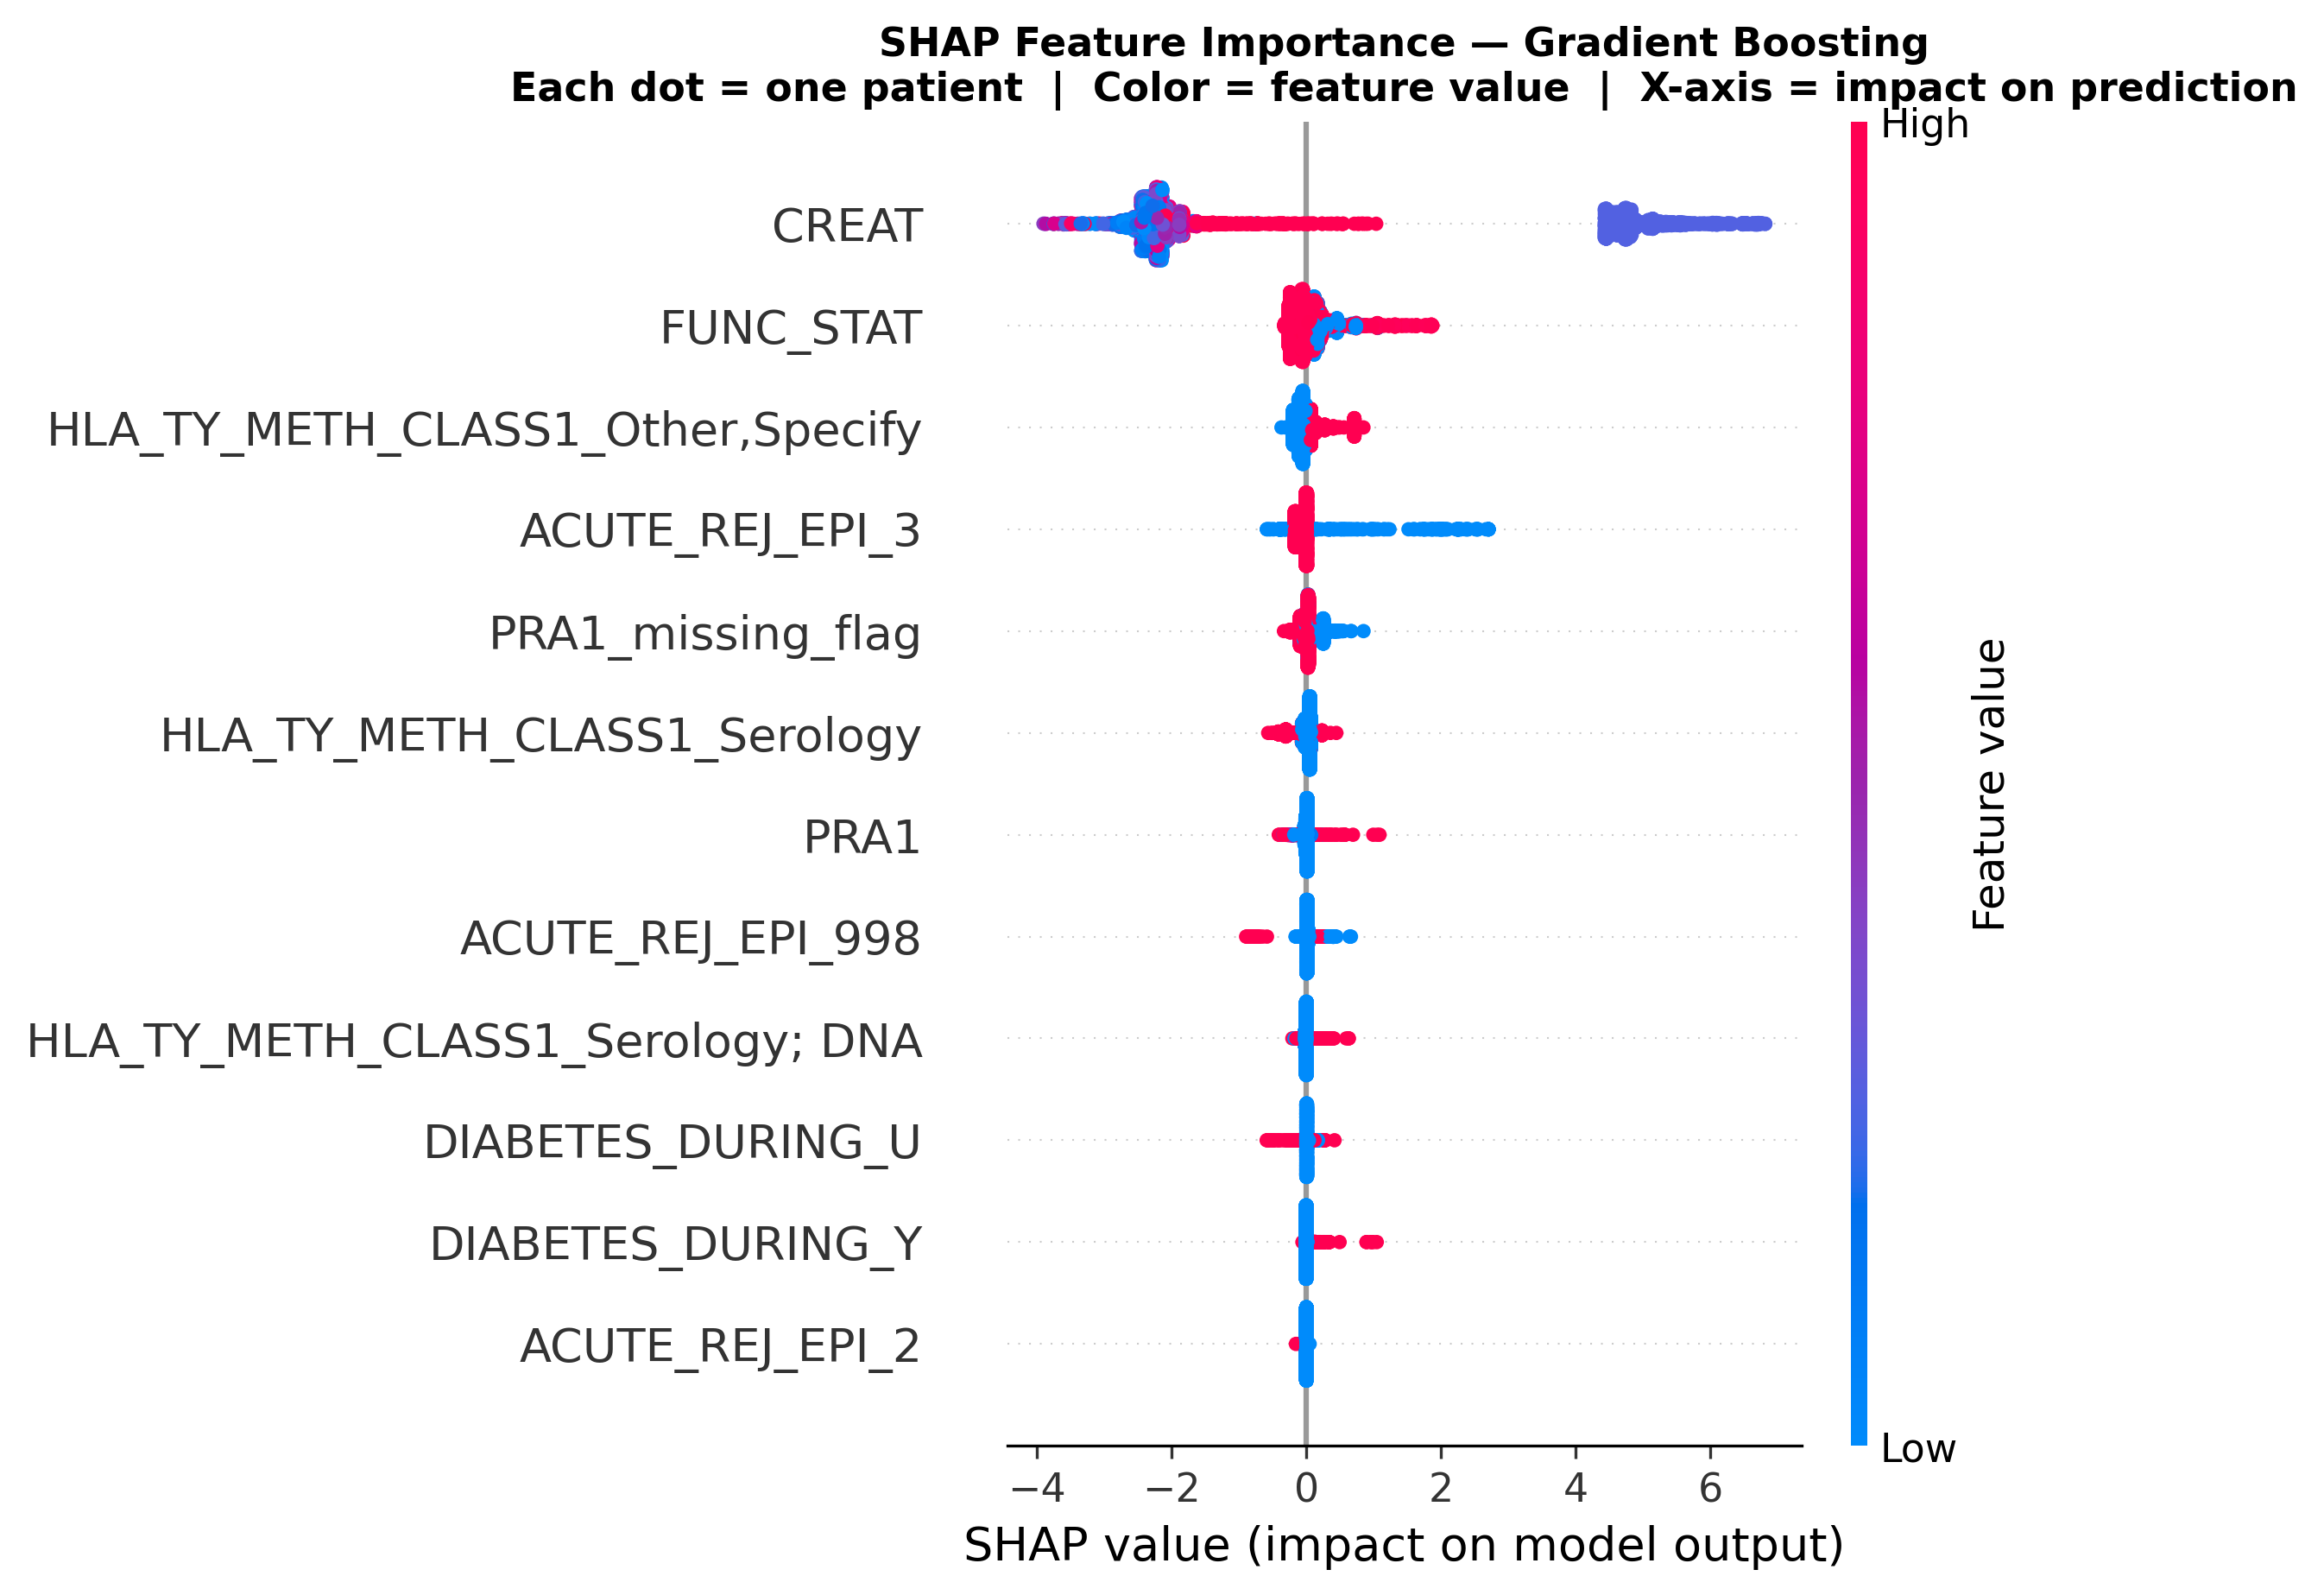
\includegraphics[width=0.9\textwidth]{step30_figures/fig1_shap_beeswarm.png}
\caption{SHAP beeswarm plot illustrating how individual features contribute to predictions across the dataset.}
\label{fig:shap_beeswarm}
\end{figure}

\begin{figure}[H]
\centering
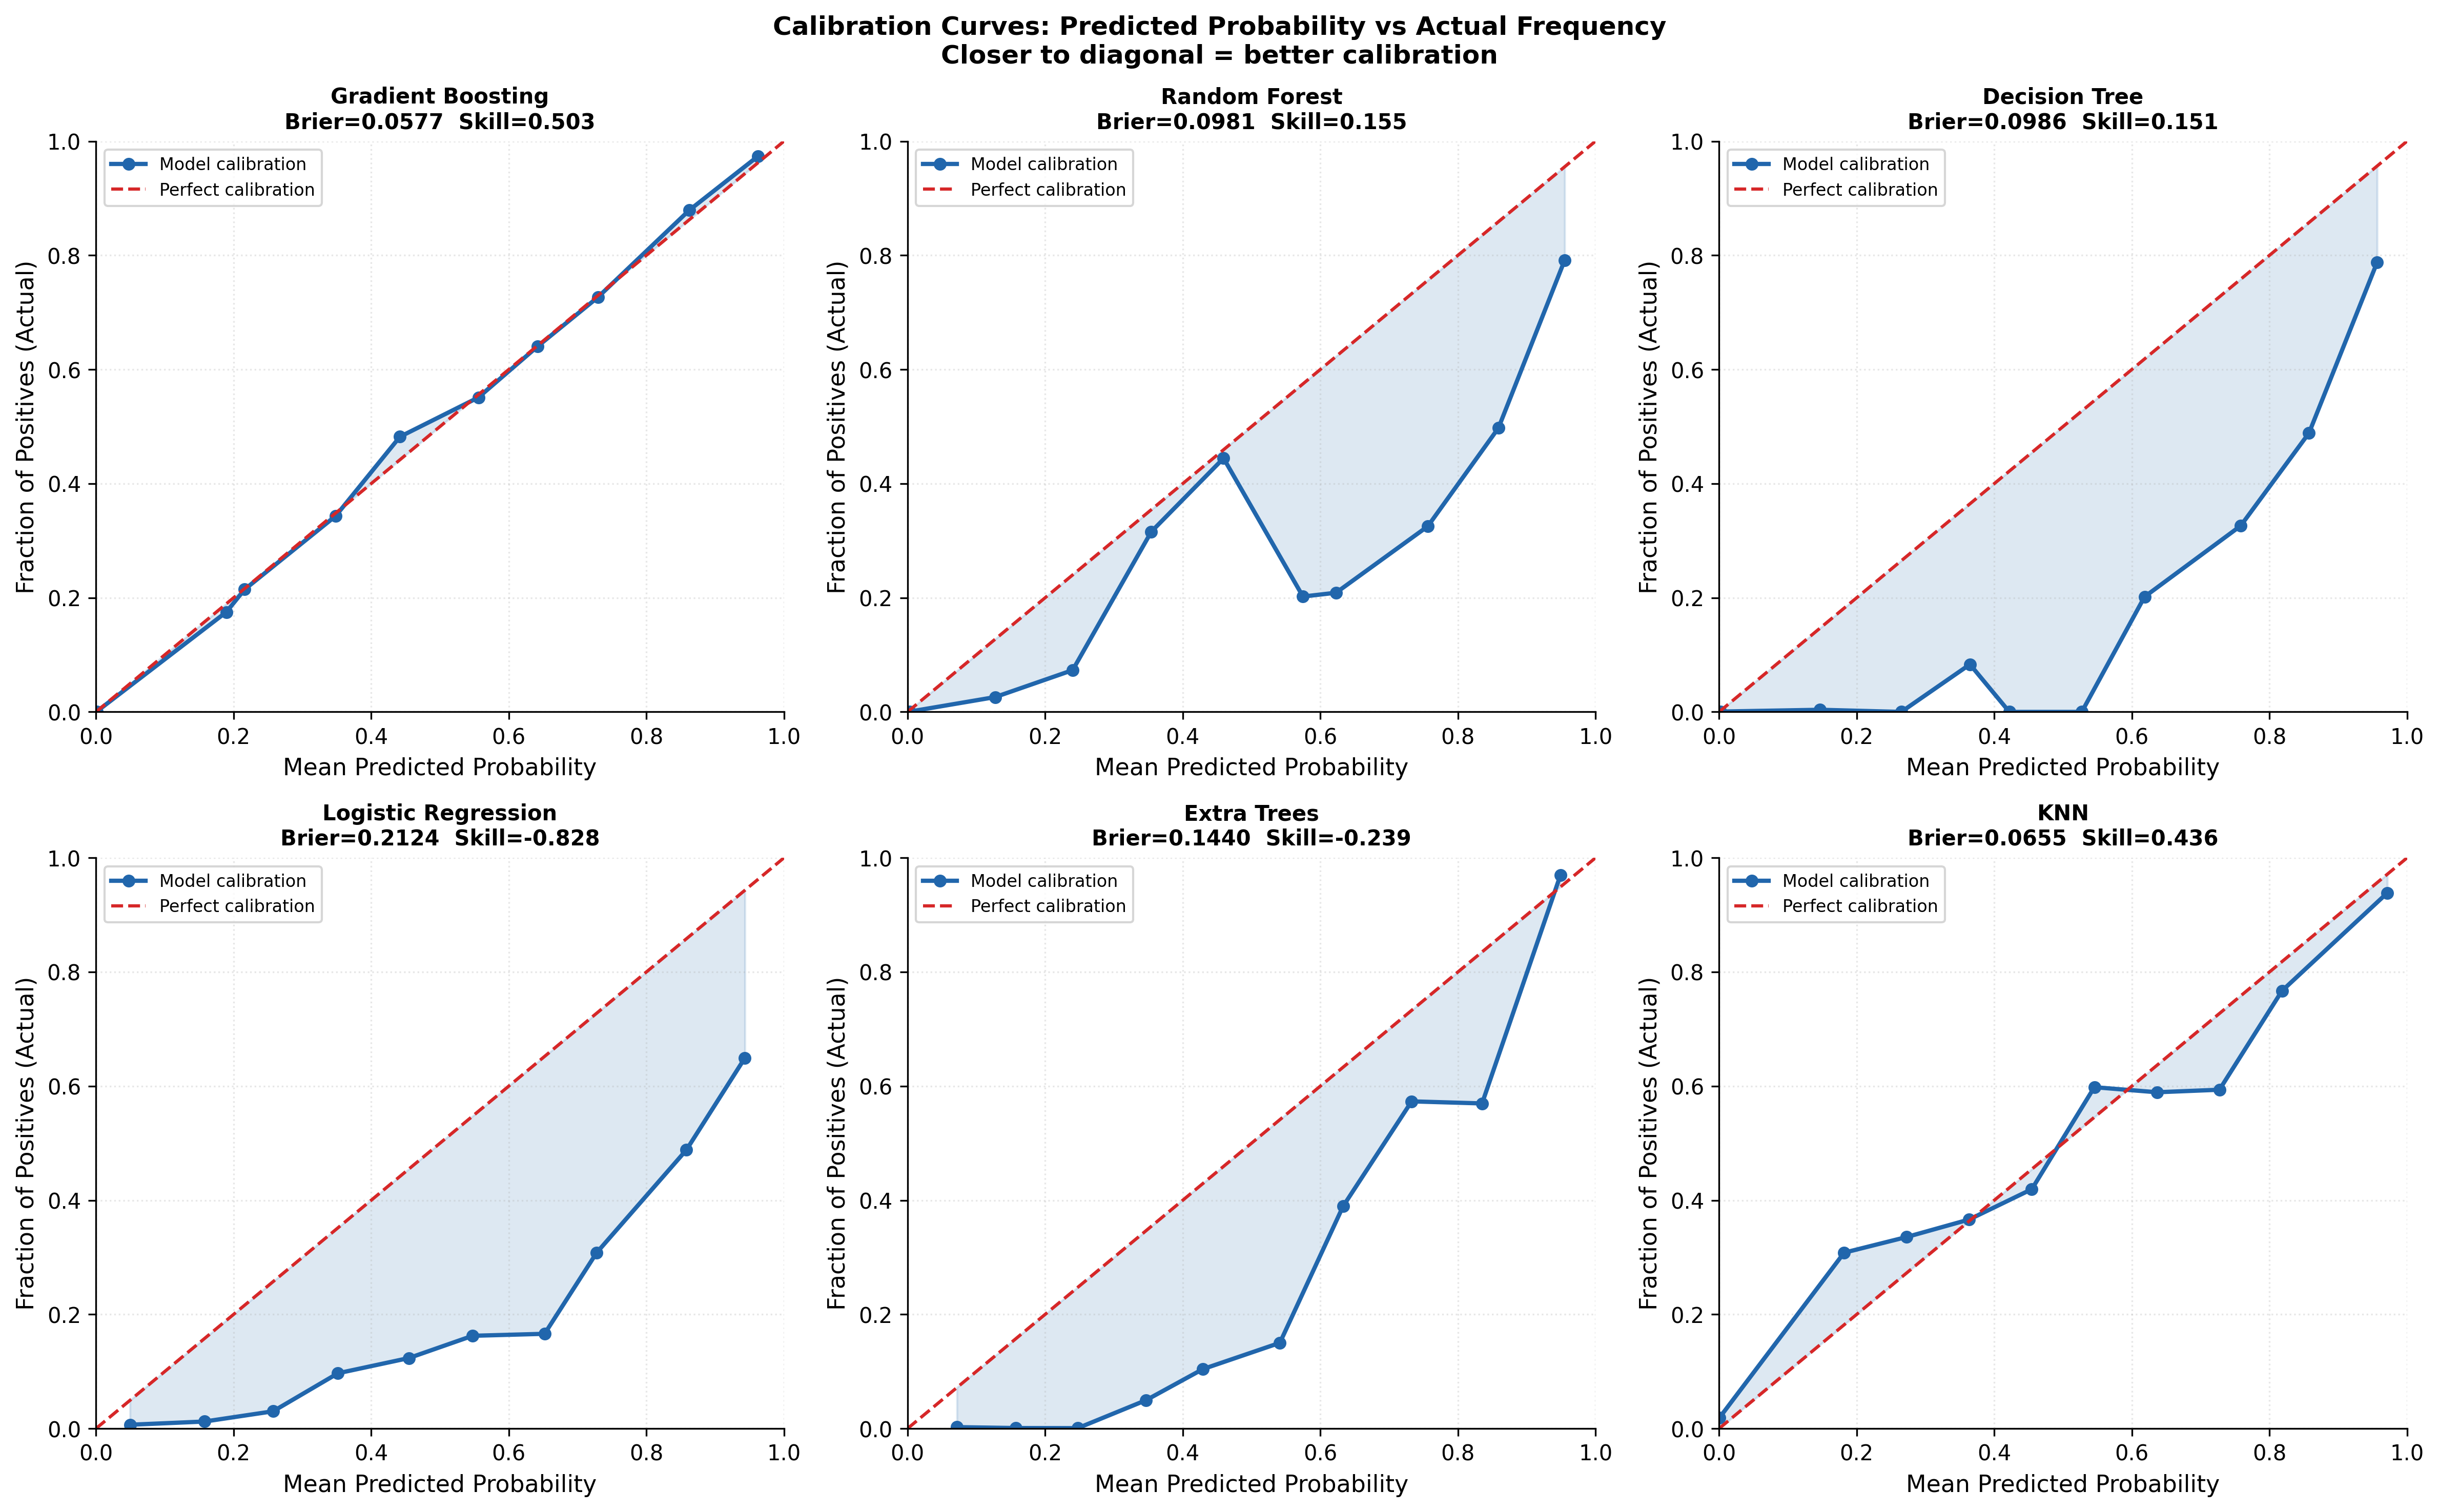
\includegraphics[width=0.8\textwidth]{step31_figures/fig1_calibration_curves.png}
\caption{Model calibration curve demonstrating agreement between predicted probabilities and observed outcomes.}
\label{fig:calibration}
\end{figure}

\begin{figure}[H]
\centering
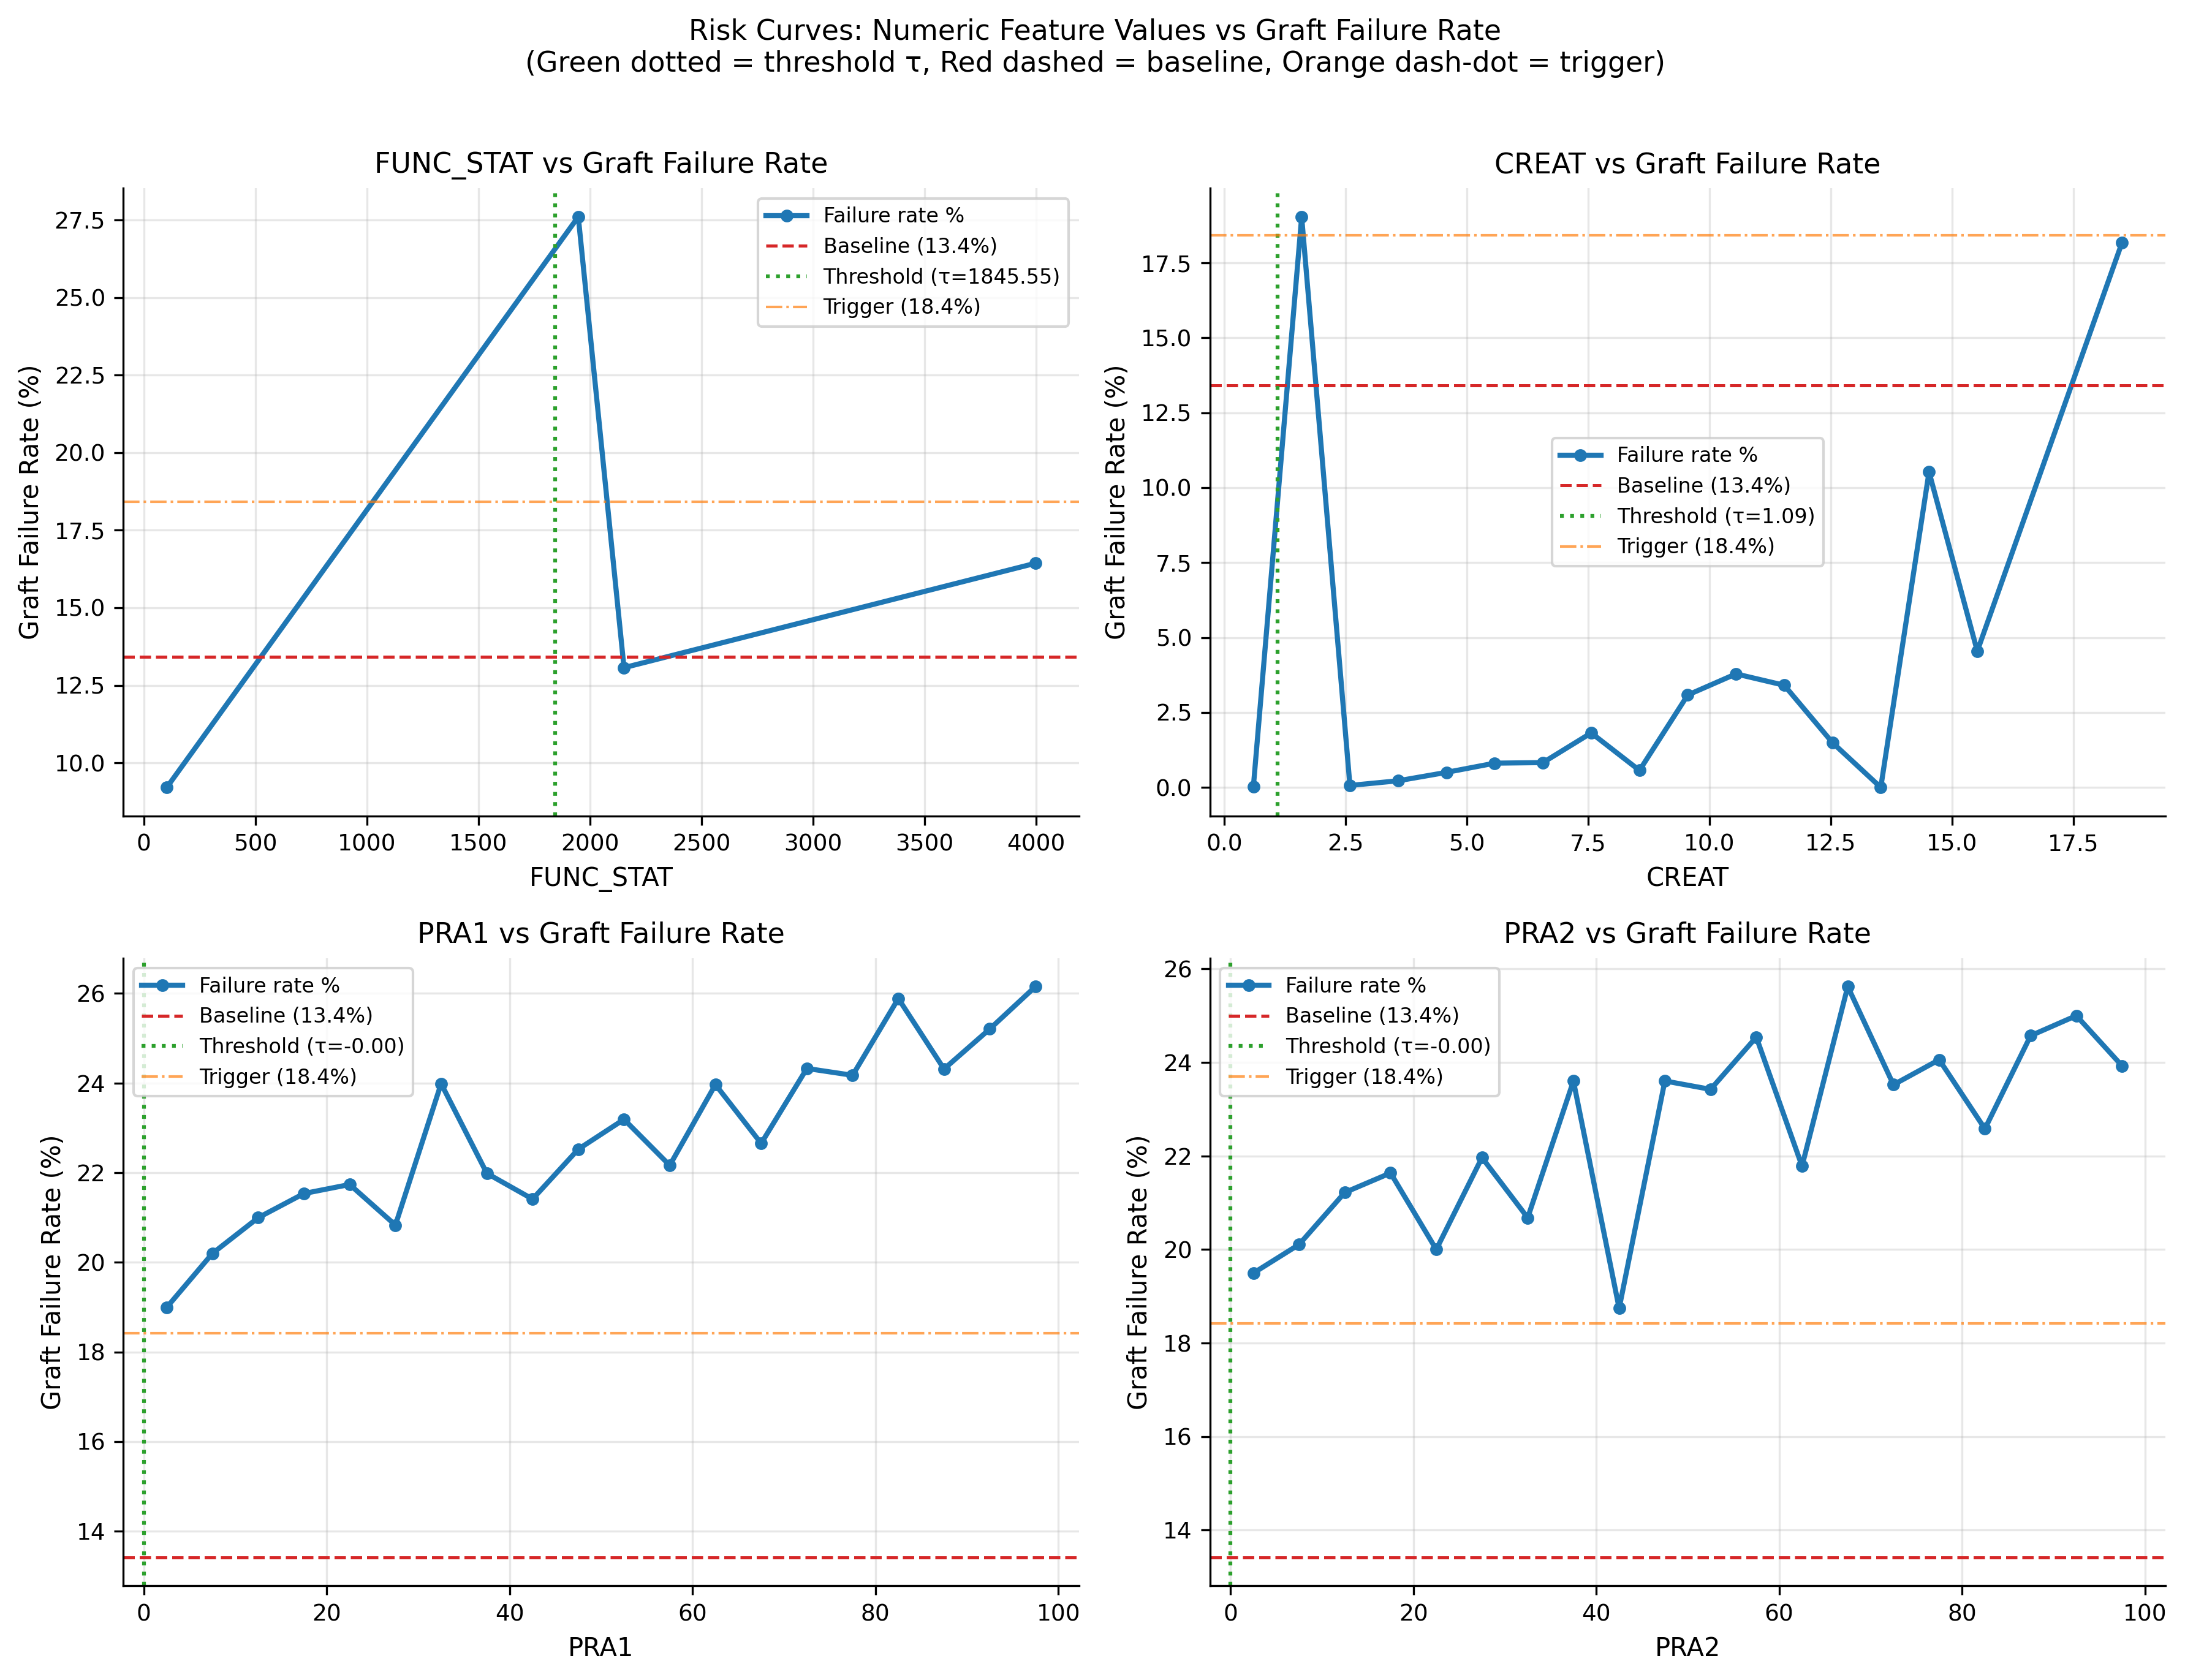
\includegraphics[width=0.9\textwidth]{step24_figures/fig1_numeric_risk_curves.png}
\caption{Clinical risk curves showing the relationship between continuous predictors (creatinine, functional status, PRA levels) and graft failure risk.}
\label{fig:risk_curves}
\end{figure}

\begin{figure}[H]
\centering
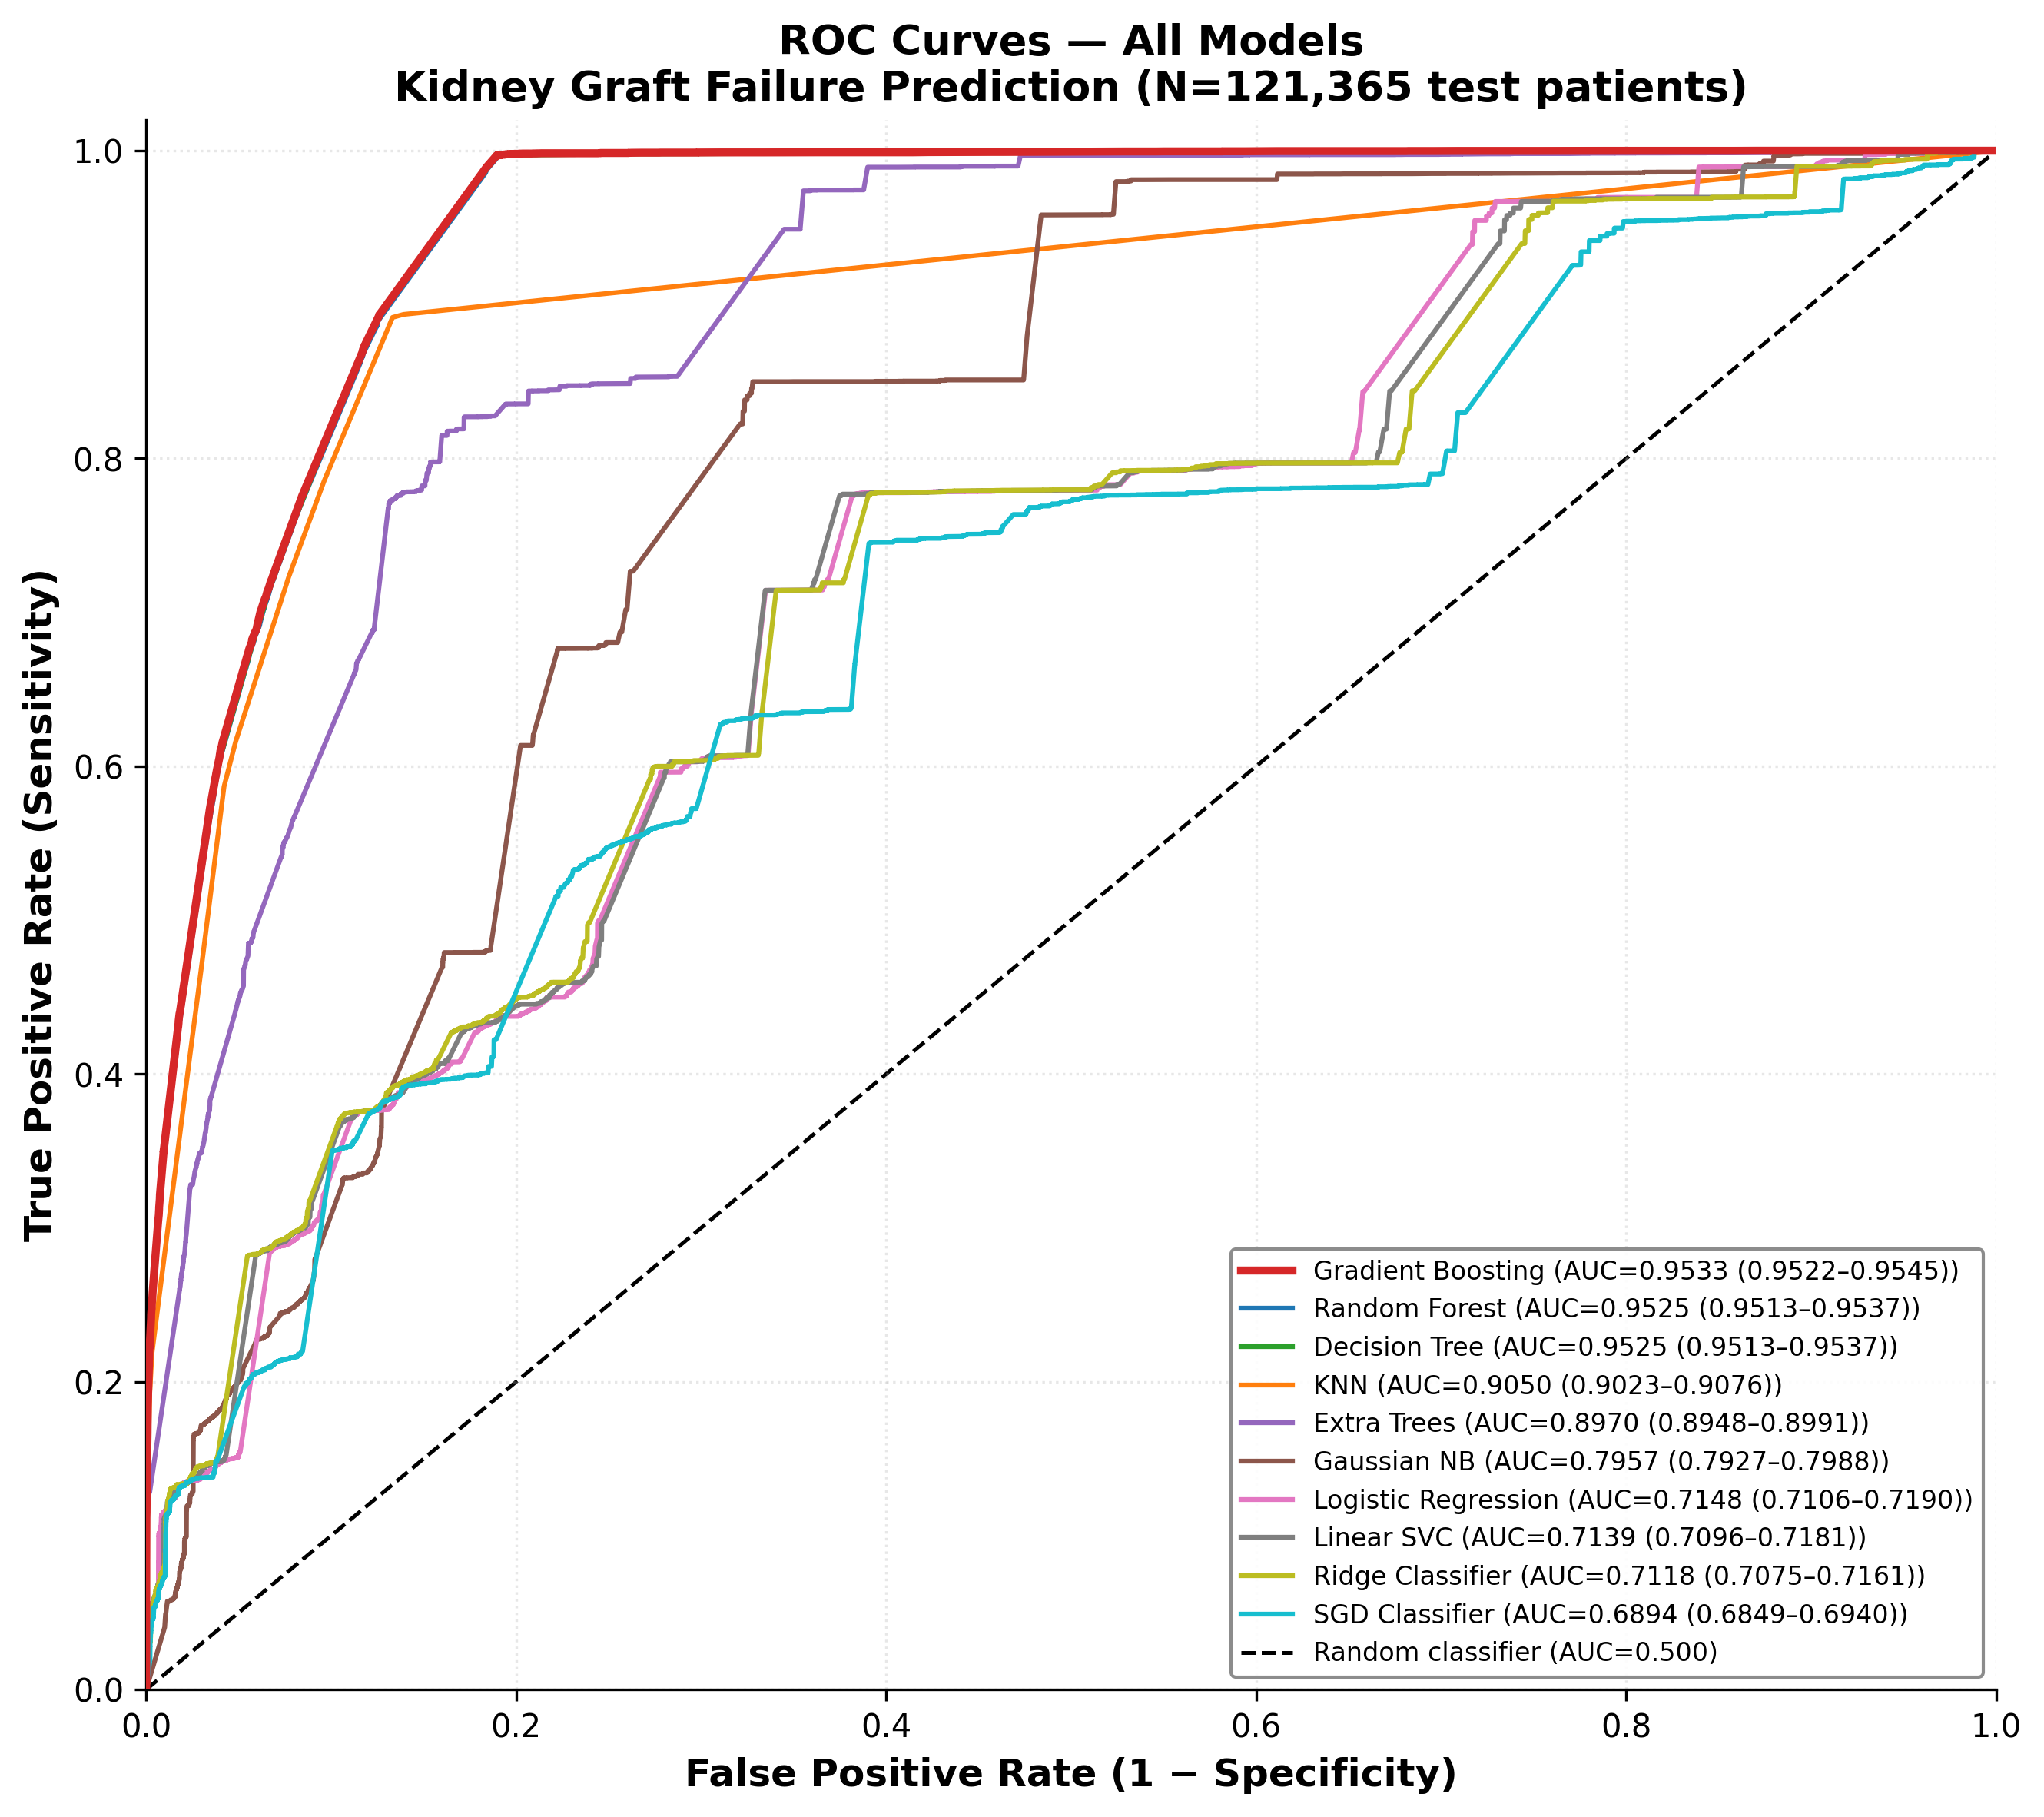
\includegraphics[width=0.9\textwidth]{step32_figures/fig1_roc_curves_all_models.png}
\caption{Comparison of ROC curves across different machine learning algorithms tested.}
\label{fig:roc_comparison}
\end{figure}

\section{References}

\bibliographystyle{plain}
\bibliography{references}

\end{document}